\documentclass[12 pct]{report}
\usepackage[utf8]{inputenc}
\usepackage{graphicx}
\usepackage[english]{babel}
\usepackage{caption}
\usepackage{subcaption}
\usepackage{float}
\usepackage{wrapfig}
\usepackage[left=1.5in, right=1.5in, top=1in, bottom=1in]{geometry}
\graphicspath{ {/Users/so/Desktop/Projects/ArRobotLearnToCodePRoject/} }
\setcounter{section}{-1}

\begin{document}

\title{%
  Alternative methods of learning using Augmented Reality\\
  \large Practical application \\
    and comparisons with other techniques}

\author{Mircea Sorin-Sebastian, coord. Cojocar Dan}

\maketitle

\begin{abstract}
The way that people acquire new knowledge and interact with the information has remained more or less the same in the modern history of humans, from paper based books to digital ebooks. The interaction with the information is practically non-existent, even more, the medium of showing the information is only two-dimensional, making the understanding of real world, three-dimensional concepts more difficult. Augmented reality, as a technology, has greatly improved in the past few years and now has the power to redesign the process of learning and teaching in ways that are still not contoured.
\end{abstract}

\tableofcontents

\listoffigures

\listoftables

\chapter{Introduction}

\section{Motivation}
On the grounds that in recent years the rate of technological advancements is increasing exponentially makes it our responsibility to always keep looking towards new ways of exploiting to the maximum the power of such technologies. Moreover when breakthroughs are powerful enough to enter into the public's attention it triggers and stimulates the desire to increase the research activity in that field, thus forming a circle that is in our interests to not break it.

As for the actual field which is the target of this study, Education, due to its major importance in forming new generations of capable people, the efforts to continuously find ways to improvise are definitely worth  it. 

\section{Objective}
The objective of this work is to find new use of recent technological advancements in Augmented Reality for the education sector and to research the effectiveness, feasibility of deploying such approaches to the general public. Also, to provide additional directions for future developments so that they enable the  forthcoming applications to have the power of redefining the already existing processes of learning.

\section{Structure}
The paper is divided into two major parts, the theoretical one that includes a description of how Augmented Reality works and the progresses that have been made in this field, followed by an in-depth depiction of the advantages that can be brought to the classical means of learning. In the second part the theoretical notions presented are applied into two applications, one being focused on the Musical domain, in more details in teaching people of all ages the basics of learning the piano and the other targeting young kids wishing to learn how to code. Both applications taking use of different types of augmented reality techniques.
\chapter{Augmented Reality}

\section{Introduction}
The meaning of the word augment is to add or enhance something. In the cause of Augmented Reality, graphics, sounds and different feedback are added into our world to create an enhanced experience.

This approach is opposite to the one that Virtual Reality takes, which is to completely replace the reality with a computer generated one.

\section{Categories of Augmented Reality}
\begin{figure}[h!]
  \centering
  \begin{subfigure}[b]{0.36\linewidth}
    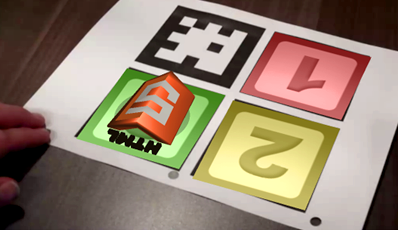
\includegraphics[width=\linewidth]{marker-based}
     \caption{Marker based}
     
  \end{subfigure}
  \begin{subfigure}[b]{0.4\linewidth}
    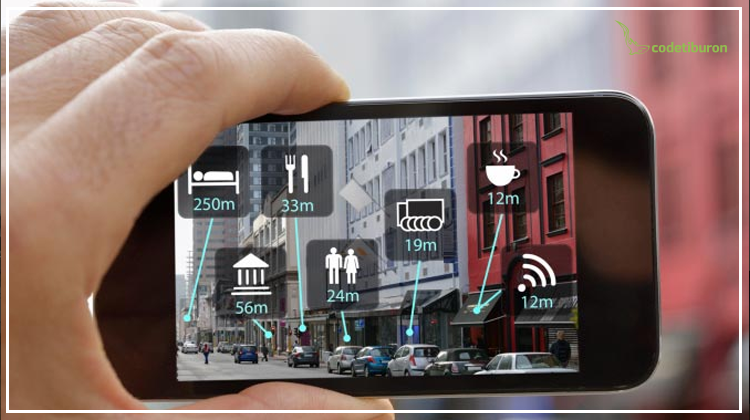
\includegraphics[width=\linewidth]{marker-less}
    \caption{Markerless}
  \end{subfigure}
  \begin{subfigure}[b]{0.4\linewidth}
    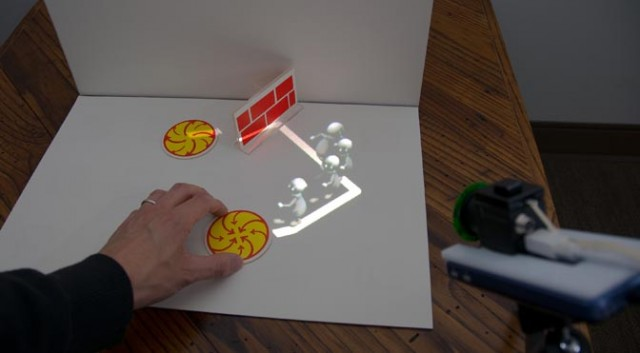
\includegraphics[width=\linewidth]{projection-based}
    \caption{Projection}
  \end{subfigure}
  \begin{subfigure}[b]{0.4\linewidth}
    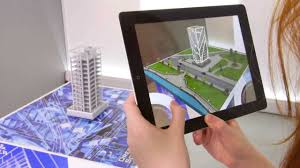
\includegraphics[width=\linewidth]{super-imposition}
    \caption{Superimposition}
  \end{subfigure}
  \caption{Categories of augmented reality}
  \label{fig:coffee3}
\end{figure}
Having their own use cases, advantages and disadvantages, several types of augmented reality approaches exist.

\subsection*{Marker based}
Uses a camera enabled device and some type of visual markers (like QR codes or certain feature points) to recognise this zones and execute certain actions like imposing a virtual object over the marker.

\subsection*{Markerless}
Also known as location-based AR, it uses GPS, digital compass, velocity meter and accelerometer to track and recognise the position of the phone, making possible the instantiation of virtual objects that appear to remain in place even if the user moves through the world.

\subsection*{Projection based}
The augmentation is realised by projecting light onto objects (the projection can also be done in mid-air with the help of laser plasma technology), though augmenting it. One use-case would be creating an interactive virtual keyboard.


\subsection*{Superimposition based}
In this approach the original view is either fully or partially replaced with a newly generated augmented view. For this to happen, the object that needs to be replaced must first be detected, so image processing plays a vital role.


\section{Types of devices}
\begin{figure}[h!]
  \centering
  \begin{subfigure}[b]{0.4\linewidth}
    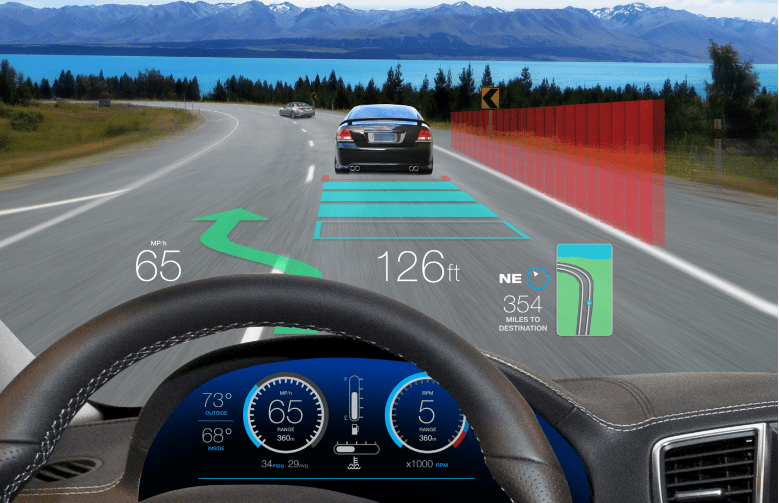
\includegraphics[width=\linewidth]{head-up}
     \caption{Head Up Display}
  \end{subfigure}
  \begin{subfigure}[b]{0.4\linewidth}
    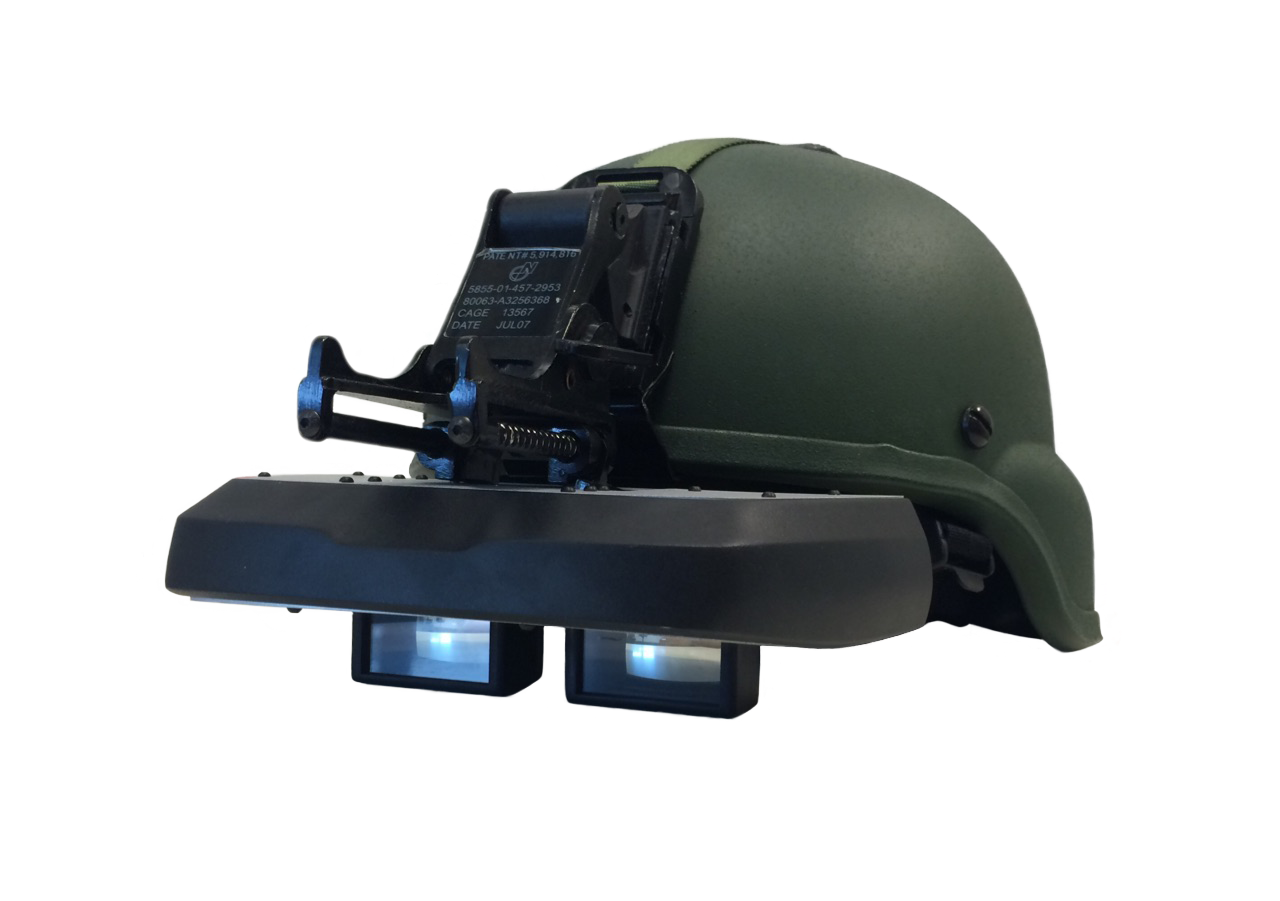
\includegraphics[width=\linewidth]{helmet-mounted}
    \caption{Helmet Mounted Display}
  \end{subfigure}
  \begin{subfigure}[b]{0.4\linewidth}
    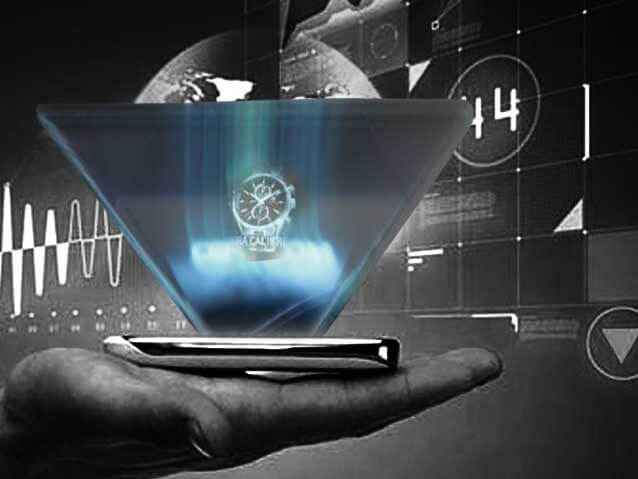
\includegraphics[width=\linewidth]{holographic-display}
    \caption{Holographic Display}
  \end{subfigure}
  \begin{subfigure}[b]{0.4\linewidth}
    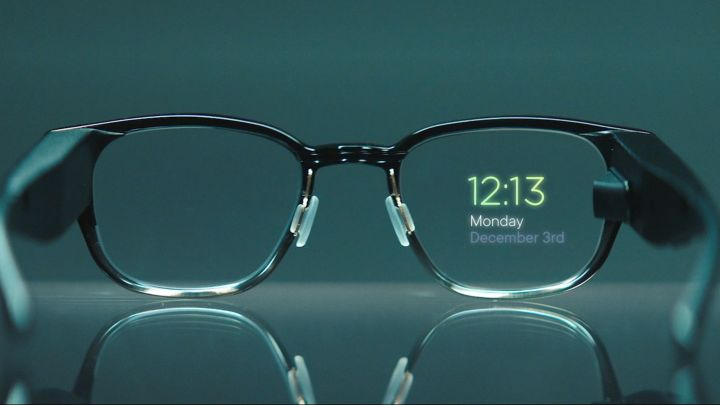
\includegraphics[width=\linewidth]{smart-glasses}
    \caption{Smart glasses}
  \end{subfigure}
  \begin{subfigure}[b]{0.4\linewidth}
    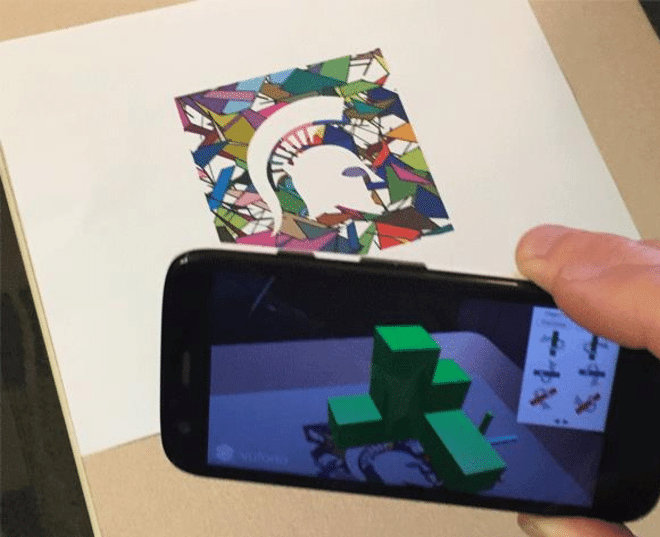
\includegraphics[width=\linewidth]{hand-held}
    \caption{Handheld}
  \end{subfigure}
  \caption{Types of AR enabled devices}
  \label{fig:coffee3}
\end{figure}

\subsection*{Head up displays}
Mainly invented for mission critical applications like flight controllers and weapon system dashboards where crucial information needs to be presented directly in the visual field of the user. In this case the projected information is collimated (parallel light rays), focused on infinity so that the user’s eyes do not need to refocus to view outside the world.
A regular HUD is composed out of a projector unit, a viewing glass and a computer that generates the data that needs to be shown.

\subsection*{Helmet mounted displays}
Represents the next logical step from the head up displays, moving the display from a fixed position to a mobile one, mounted directly on the helmet.

\subsection*{Holographic displays}
They use light diffraction to generate three dimensional forms of object in real space

\subsection*{Smart glasses}
As the use case of Augmented Reality transitioned from critical application (mostly used by army) to  applications available for the general mass of user, helmet mounted displays shifted toward a lighter form-factor, integrated directly in smart glasses. 

\subsection*{Handheld AR}
The majority of mobile devices enter in this category, as both major mobile software providers, Apple and Android offer augmented reality support (ARKit and ARCore). The advantage of this approach is that it makes augmented reality accessible to anyone with a decent smartphone, the drawback being the fact the user experience is not always satisfying as you need to to always hold and pin-point the device towards the zone you want to interact with.

\section{ARKit}
Primarily it does three essential things behind the scenes: tracking, scene understanding, and rendering, thus taking the heavy lift from the developer (as you only need to anchor virtual objects to the real world, and they stay glued to the physical position they were placed).

ArKit uses a technique called visual-inertial odometry (VIO). In more details, the position of the phone is tracked via the Visual system (camera), by matching a point in the real world (called feature point) to a pixel on the camera sensor for each frame. In parallel the pose is also tracked by the Inertial system  (also called IMU) formed of an accelerometer and gyroscope. These two outputs are combined via a Kalman filter to determine which of the two system provides the best estimate of the real position.

\begin{figure}[]
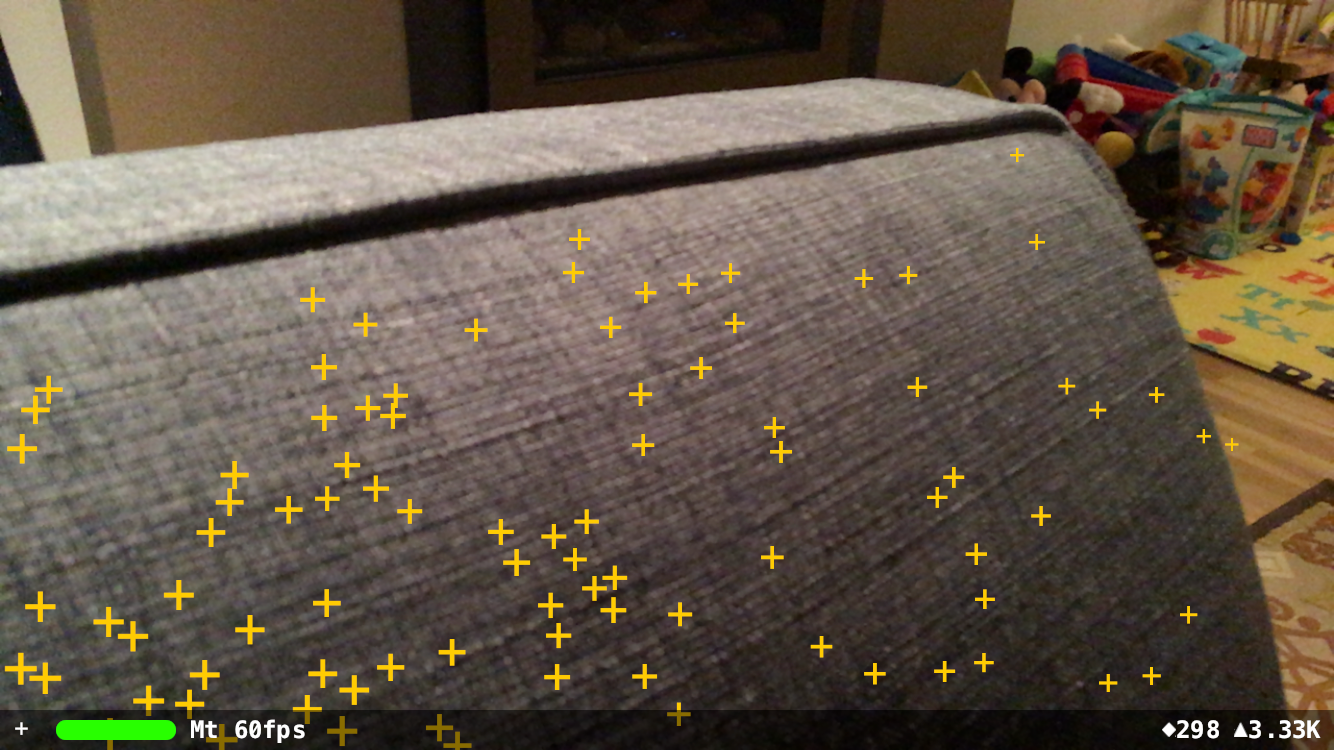
\includegraphics[width=1\textwidth]{feature-points}
\centering
\label{fig:feature-points}
\caption{ARKit feature points}
\end{figure}


The Visual system is refreshed every time a new frame is captured by the camera (30 times per second), while the inertial system outputs 1000 readings per second. Both the systems alone would accumulate errors in certain condition, but the fact that there are no interdependencies between them leads to an overall much better performance. For example, the visual systems outputs weak results if the image is shaken, if the light is weak or the targeted object has a smooth surface (without particularities, like glass, or a perfectly white wall), during this time the Inertial part carries the load, and vice-versa in the case that the device is still (so there is no inertial data), the camera has the possibility to capture more accurate data, thus receiving priority as being closer to the truth from the Kalman filter.




\subsection*{Plane detection}
\begin{figure}[H]
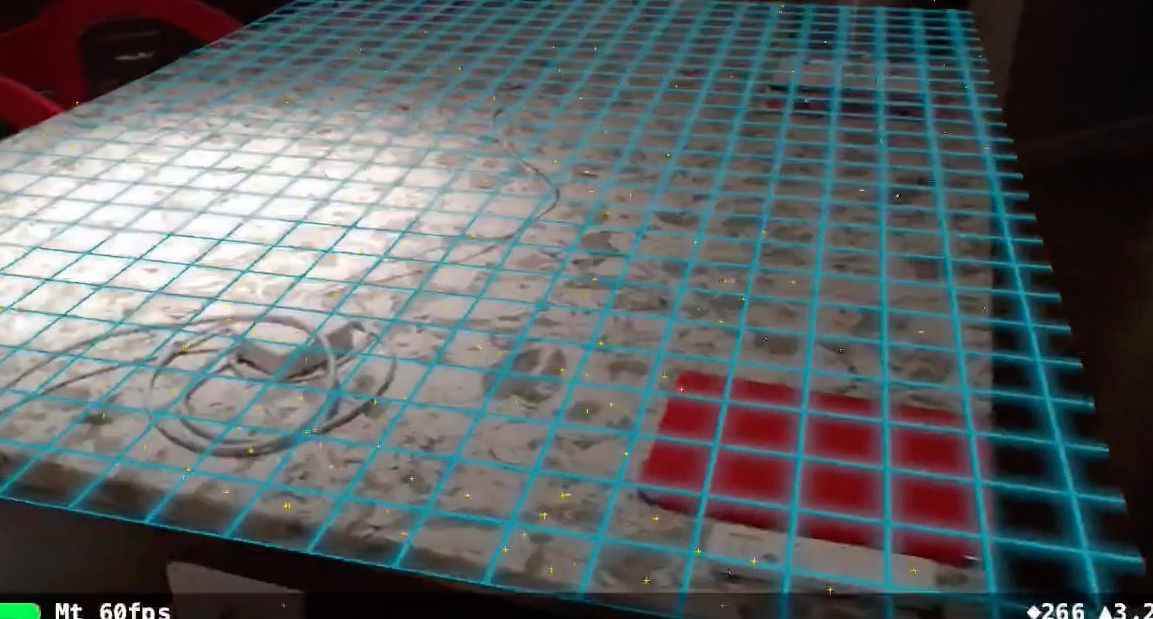
\includegraphics[width=1\textwidth]{plane-detection}
\centering
\label{fig:plane-detection}
\caption{ARKit plane detection, spawning blue squares}
\end{figure}

In order to create an AR experience that can blend with reality, the ability to place an object on the ground represents one of the critical requirements. 

This can be achieved using the feature points detected by the Visual system, each three points are considered to define a plane, and after doing multiple such calculations, the plane that represents the ground can be estimated.

\chapter{Improvements in learning by using Augmented Reality}
\section{Introduction}
According to Shapley et al. (2011), lessons that are supported by technology will lead to more innovative forms of teaching and learning. This is because the use of technology involves real-world problems, current informational resources, simulations of concepts, and communication with professionals in the filed. In addition, learning using technology is believed to complement the traditional forms of teaching and learning (Yasak et al., 2010)

In recent years, as augmented reality emerged as a new technology, its potential for applications in education was discovered and the interest grew constantly. In research conducted by Teoh and Neo (2007), the respondents reported that it was boring to just hear the lecturer talking in front of them. The students believed that the integration of technology would help them in their learning process. 

\section{Impact of using Augmented Reality in learning}
One of the aspects that discourage future students in following a science path is the thought that grasping abstract aspects it is going to impose them real problems. The majority of difficulties that appear are related with understanding multi-dimensional data.

Augmented reality is a great way of visualising three-dimensional objects, as it replaces classical wood or cartoon physical shapes that are used by teachers with virtual, augmented objects. Also, there are situations that not only require a three dimensional way of showing objects, but to also provide a way to observe dynamical interactions with the studied item.

The use of AR would also increase the time that students can spend studying different objects that otherwise would only be accessible inside the school hours, thus providing an unrestrained amount of study time.

\begin{table}[H]
\centering
 \begin{tabular}{||p{20mm} p{30mm} p{40mm} p{30mm}||} 
 \hline
 Author/s & Field & Purpose of AR Use & AR Features Used \\ [0.5ex] 
 \hline\hline
 Chang et al. 2011) & Medical education (surgical training) & To provide training and to plan and guide surgical procedures & AR image-guided therapy \\ 
 Yeom (2011) & Medical education (anatomy) & To teach and test anatomy knowledge (of the abdomen in particular)  & nteractive 3D anatomy pictures and haptic feedback \\
 Hedegaard et al.(2007) & Medical education using the electrocardiogram (ECG/EKG) AR system (called the EKGAR system) & To extend medical students’ spatial awareness in relation to specific myocardial diseases by enabling users to navigate through and slice open 3D representations of a patient’s heart & Vision-based 3D tracking technologies and interactive features \\
 Singal et al. (2012) & Chemistry education & To provide an efficient way to represent and interact with molecules, leading to a better understanding of the spatial relation between molecules & AR technology for exhibiting the models \\
 Cerqueira and Kirner (2012) & Mathematics & To teach geometry through the use of 3D geometrical concepts & Head-mounted display and personal interaction panel  \\ 
 Mathison and Gabriel (2012) & Biology (School in the Park project) & To teach participants that habitats are connected like links in a chain (food chain) & AR experience  \\
 Coffin et al. (2008) &  Physics & To overlay graphics on top of the physical props to visualize these forces (speed, velocity, acceleration, pressure, friction, energy changes) invisible to the human eye  & Augmented video, videoconferencing, tracked physical props (e.g. toy cars) \\
 Fleck Simon (2013) & Astronomy  & To show augmented views of the celestial bodies and support learning using spatial visual guides and views from a terrestrial observer & AR learning environment \\
 Martin et al. (2011) & History & To gather information and enhance the experience of visitors to cultural organisations (museums and games archaeological sites) & Mobile AR educational \\
 \hline
 \end{tabular}
  \caption{Meta-analysis of research on the use of AR in different fields of education. Cited from  \cite{note1}}\label{tab:a}
\end{table}


\section{Pitfalls and limitations}
It is known that designing an application that actually improves the process of learning (no matter the form and the device it is running on) in a certain field is a task that requires serious research as usually these kinds of solutions are not that intuitive to use, for both teachers and students. 

From other technologies, AR's advantage is the fact that it offers a hands on approach by integrating it's interactions capabilities directly with the reality (in forms of holograms), thus theoretically closing the gap between real life teacher driven learning and text-book based classical learning. This advantage comes with a price, as latter forms of e-learning have been present and researched for years now, they have come to a more mature stage, some of them ready to enter in student's life, but as AR approaches have the power to redefine everything, they have to catch up in making sure that these kinds of solutions are straightforward, thus simplifying the process of learning, not making it more complex.

From a technological point of view, only with the progress of software and hardware from the past few years AR has became feasible enough so that it can reach a large audience of people. At the moment, mobile devices (Hand-Held AR) are the only one that can bring AR to the masses, with only the majority of high-end phones and tablets launched in the past year and the half, having AR capabilities. The other types of AR (like smart glasses) would offer a more immersive approach, but the cost of these devices (HoloLens by Microsoft) makes them available only for companies and research purposes.



\chapter{Application in Musical domain}

\section{Problem}
The importance of playing a musical instrument is indisputable, even as a side hobby, learning how to do such a thing provides real benefits to the life of an individual. Unfortunately, for people which do not possess basic musical theoretical background, learning a musical instrument seems a hustle and is often abandoned from early stages. Even if this step is passed the amount of people who are self thought is small and benefiting from the services of a music school can be expensive or disruptive. 

\section{Related work}
\begin{figure}[H]
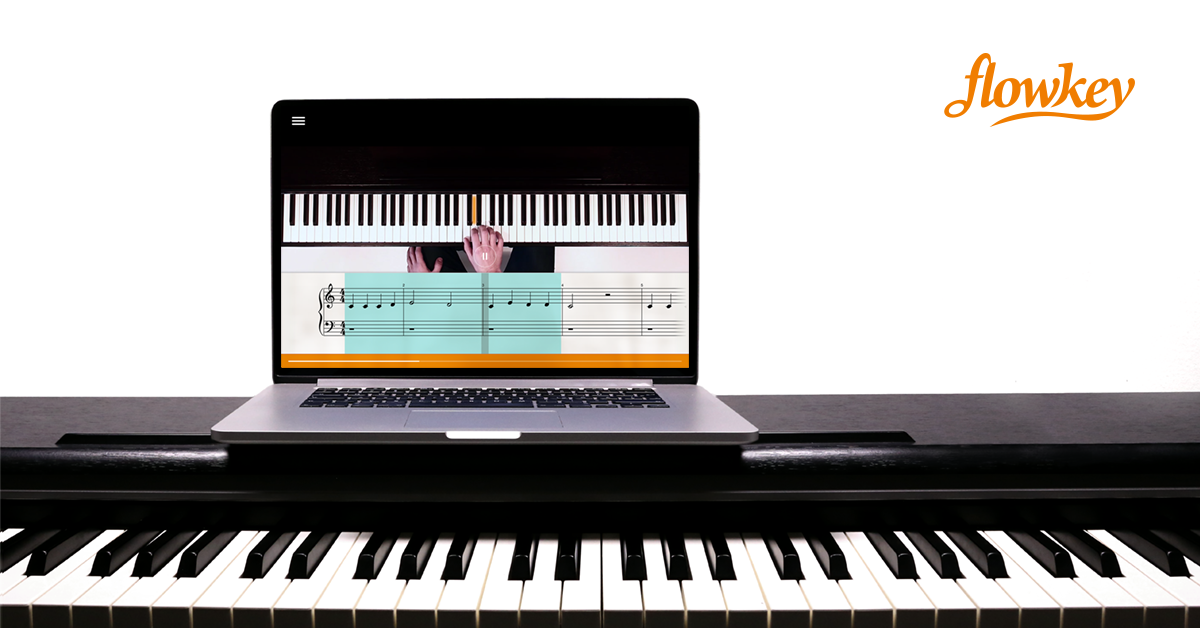
\includegraphics[width=0.7\textwidth]{flowkey}
\centering
\label{fig:hololens}
\caption{Flowkey concept}
\end{figure}

Applications like FlowKey and Piano Maestro dominate the section of self learning piano playing. They work by continuously tracking the keys that are pressed (either by listening to the generated audio or by directly connecting the piano to an external computer). By using a screen that can be be in a form of either a phone or a laptop, additional information can be rendered: the progress you are making, the accuracy, tips on which fingers to use and one of the most important, the musical sheet (that can be simplified for beginners understanding).


The other category of applications involves a more virtual approach by eliminating the need of having a physical piano or an organ, they allow versatility at the cost of loosing the real tactile feedback and experience. These kinds of solutions are more suited for entertainment rather than having actual educational value.

\section{Solution}
\begin{figure}[H]
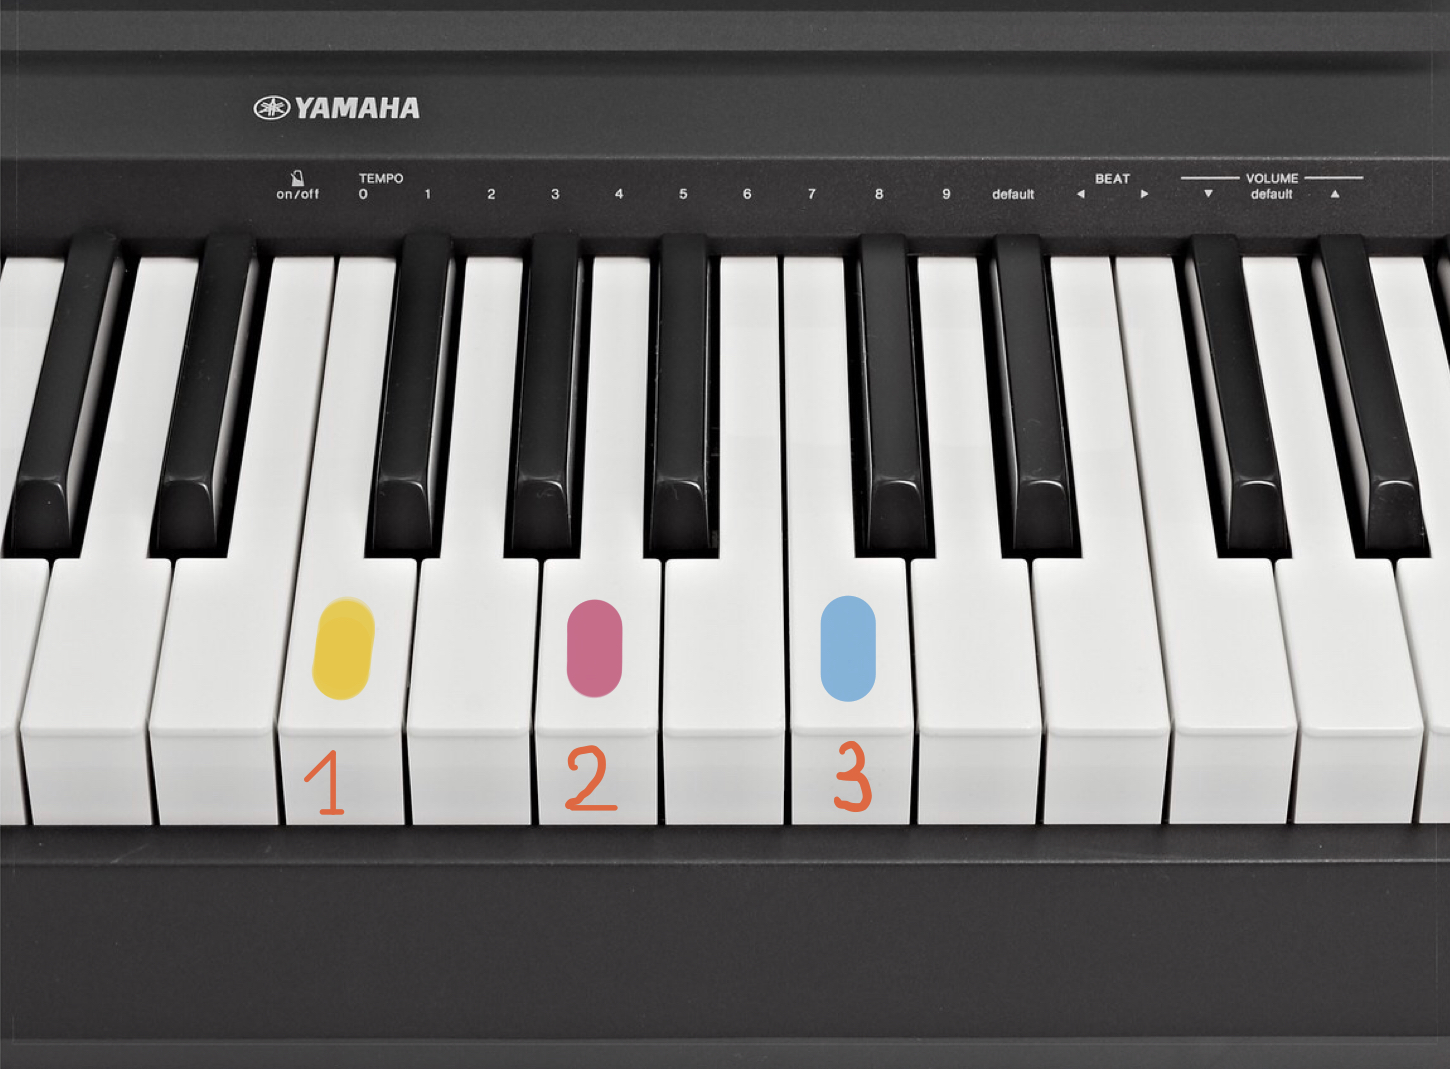
\includegraphics[width=0.7\textwidth]{piano}
\centering
\label{fig:feature-points}
\caption{HoloPiano Concept Demo}
\end{figure}
HoloPiano represents an application dedicated for people that are eager to learn the basics of piano playing. It uses Augmented Reality to show holograms over the keys that need to be pressed.



\begin{figure}[H]
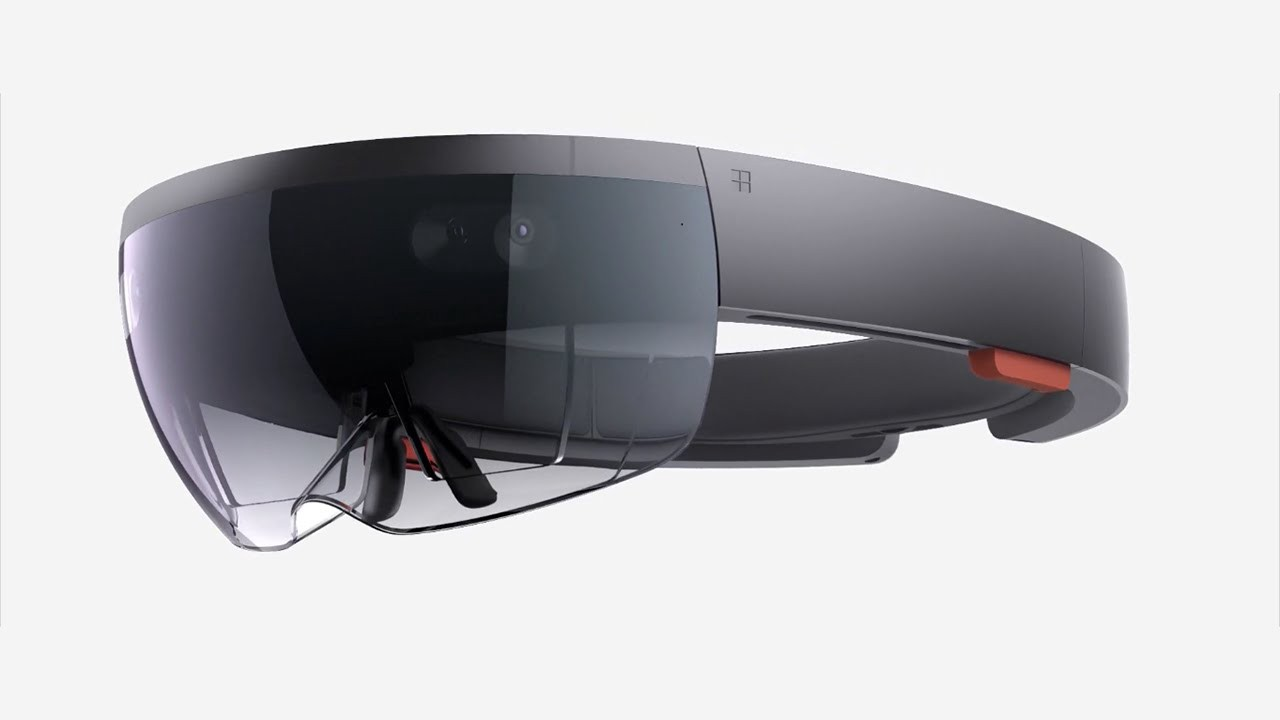
\includegraphics[width=0.7\textwidth]{hololens}
\centering
\label{fig:hololens}
\caption{HoloPiano from Microsoft}
\end{figure}



The device on which it is running on (as the name of the application probably hints to) is the first generation of HoloLens augmented glasses built by Microsoft.


In this case, augmented reality offers an unique approach for learning, allowing also people who do not have an extensive musical background to learn directly by doing, by approaching and mastering different plays in order of their difficulty, grasping dexterity, and theoretical background simultaneously.

We headed towards an augmented approach (instead of a virtual reality one) due to the fact that it was a solution that would offer the actual tactile feedback that only a real piano key can provide. Moreover, as there are a multitude of piano and organs, all with different key sizes and specs (including low end, beginner purposed instruments), the capability to learn directly on the device you own, directly from the comfort of your own house represents a plus.

\section{Architecture}

\begin{figure}[H]
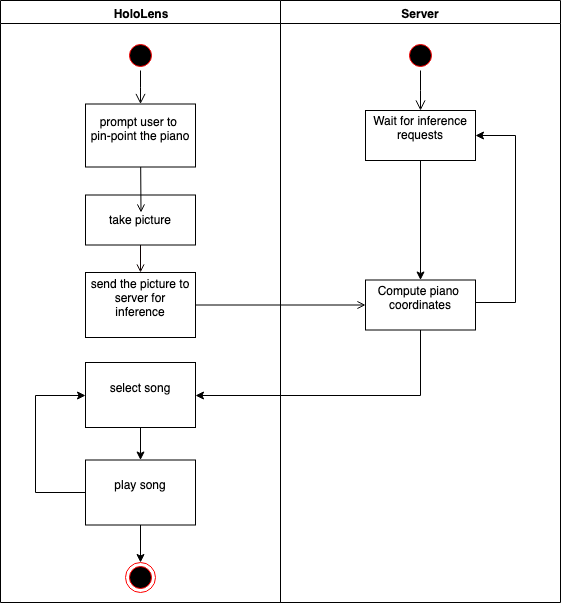
\includegraphics[width=0.9\textwidth]{HoloPianoStateDiagram}
\centering
\label{fig:feature-points}
\caption{ARKit feature points}
\end{figure}

The flow of the app is the following, after startup, for more easy computing the device is going the ask the user to pinpoint the corners of the piano (look at each corner and make a pinch gesture), when the piano is incapsulated correctly, along with this data HoloLens is going to take a camera snapshot and send everything to a server where the position of each keys are going to be inferred, sent back and mapped by the HoloLens. From this point the user can select a song base on its difficulty and start the process of playing (where holograms are going to be spawned up on the keys that are needed to be pressed).

An initial approach consisted in creating a Convolutional Neural Network that would infer the position of the piano and all its keys (without prompting to the user for specifying the pianos corners), but the first generation of HoloLens doesn't have support for running inference locally.

As a backup solution we had chosen to prompt for those corners and with image processing to just infer the position of all keys (as the application is designed to support multiple piano configurations), process that is not as computing intensive as a convolutional neural network.

\subsection *{Detecting the piano keys}

\begin{figure}[H]
  \centering
  \begin{subfigure}[b]{0.8\linewidth}
    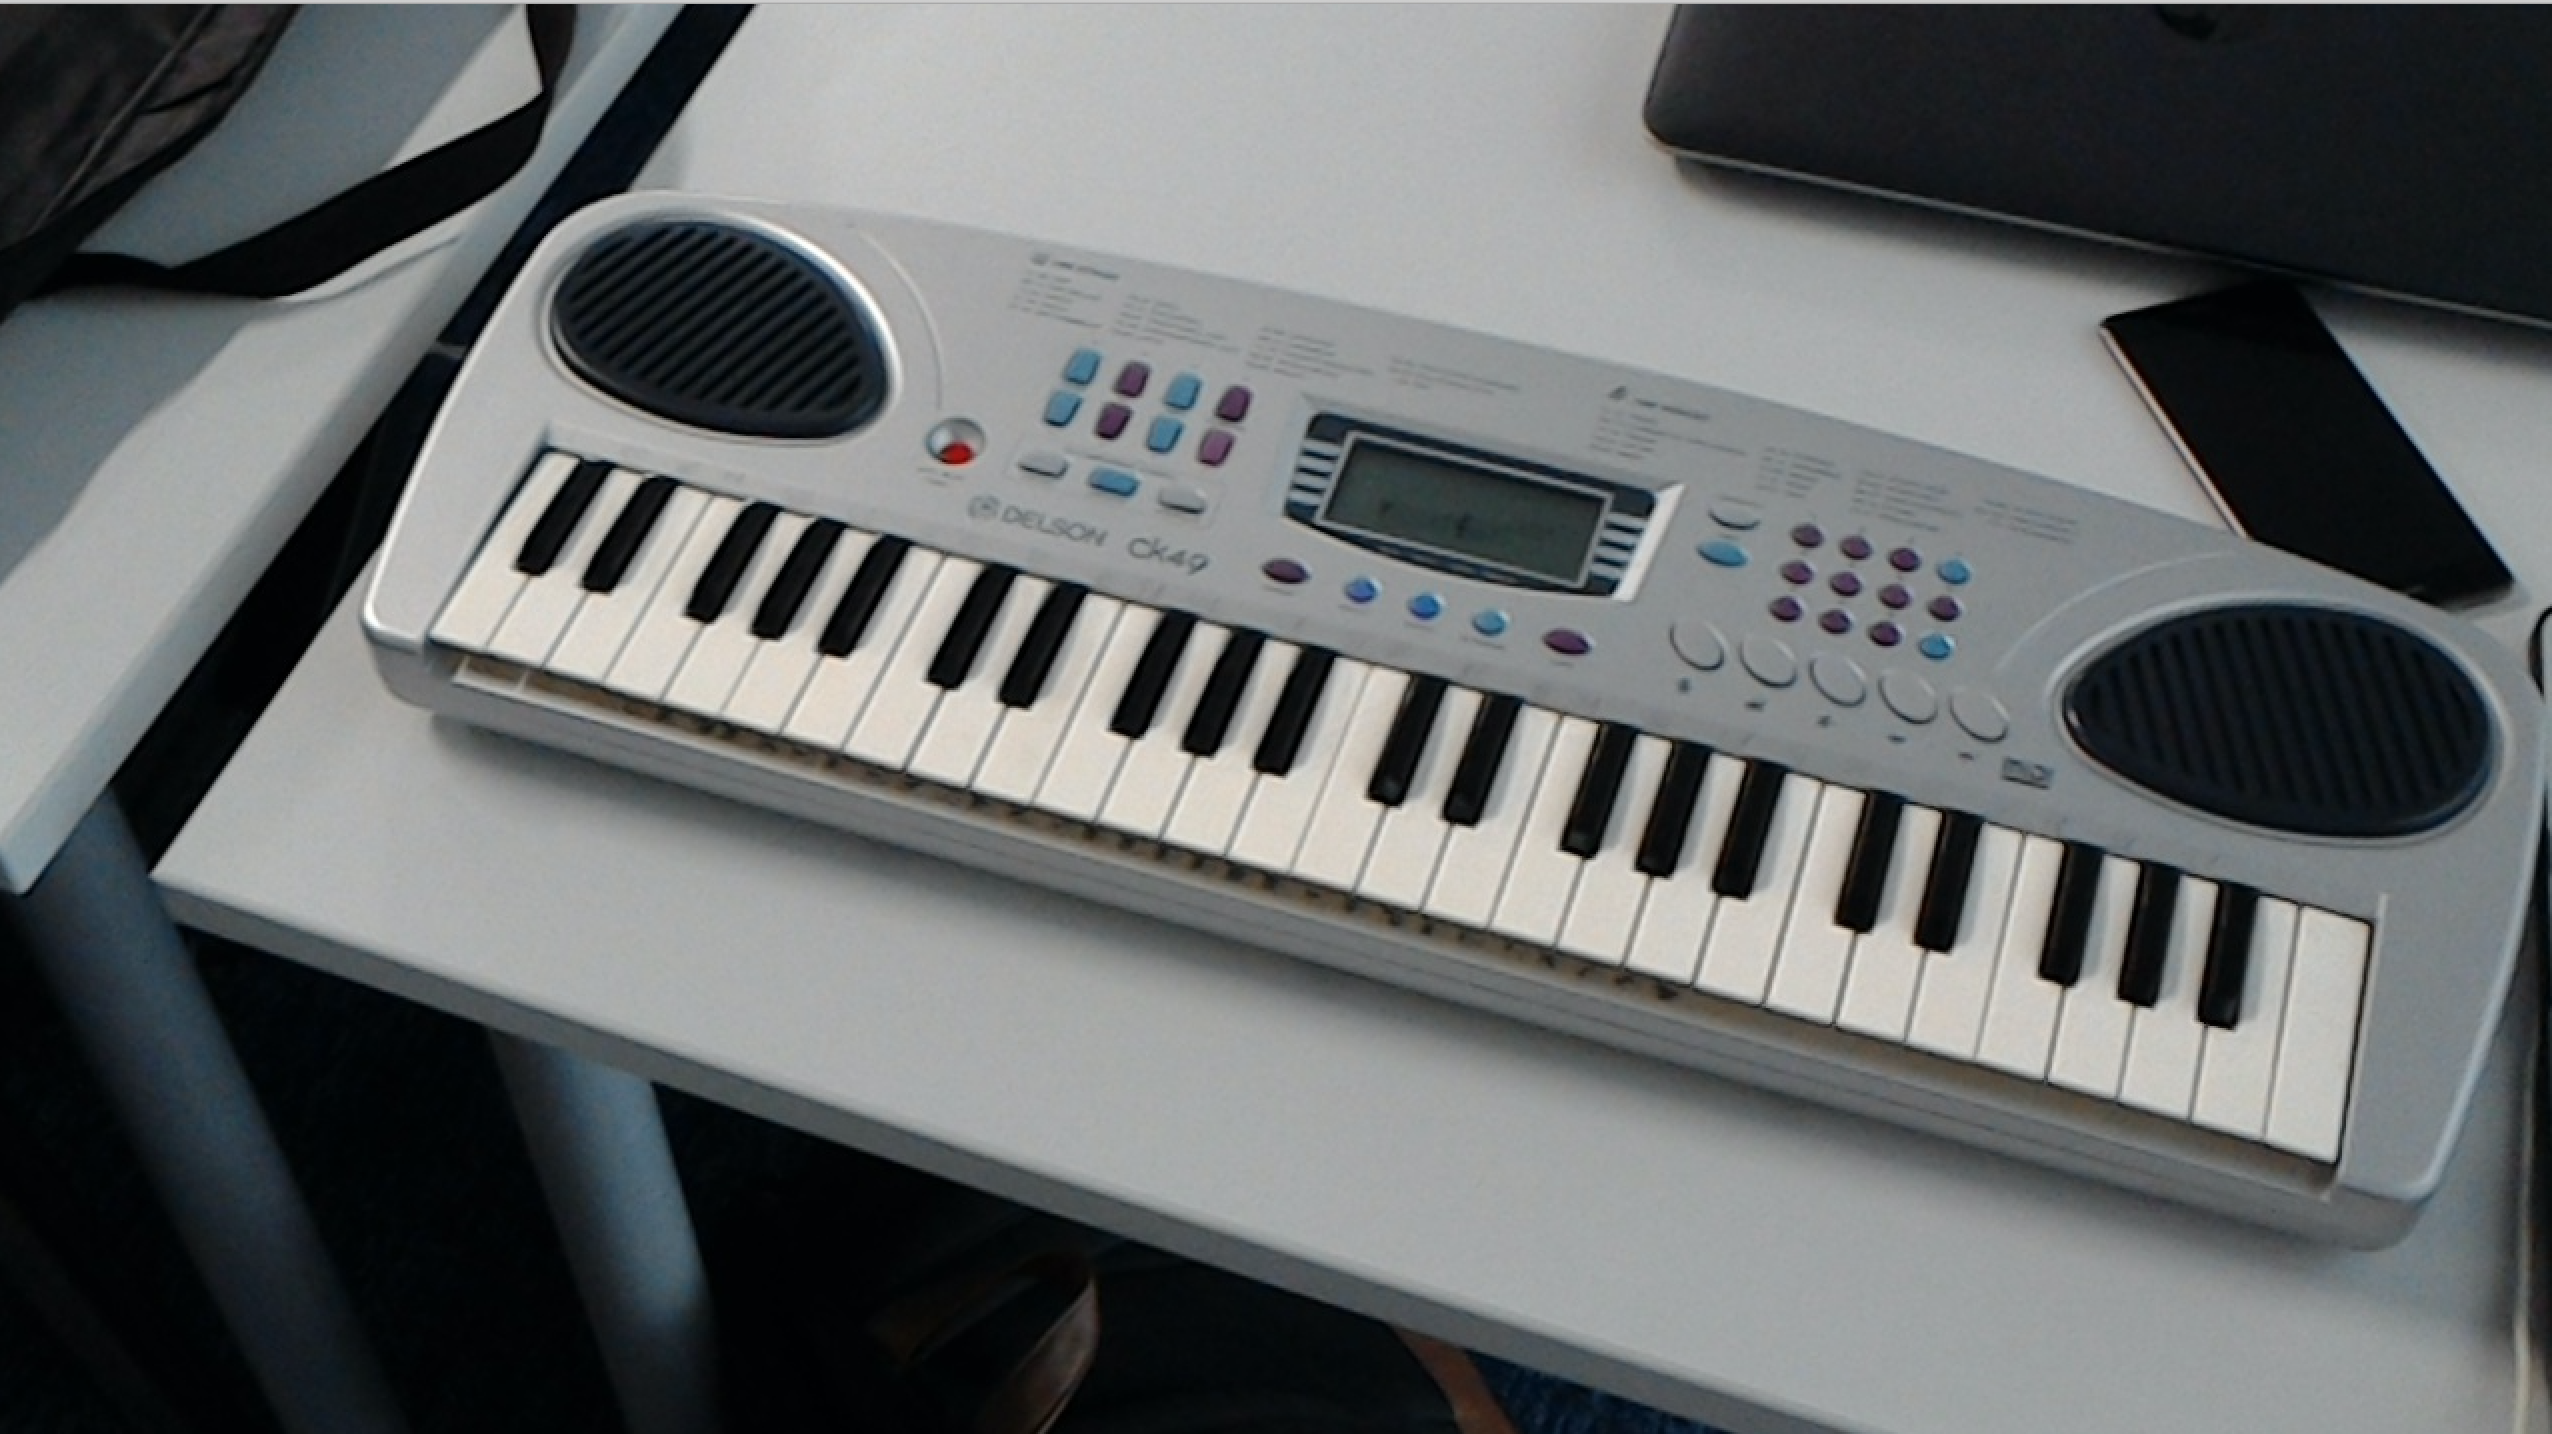
\includegraphics[width=\linewidth]{piano-original}
     \caption{Original Image}
  \end{subfigure}
  \begin{subfigure}[b]{0.8\linewidth}
    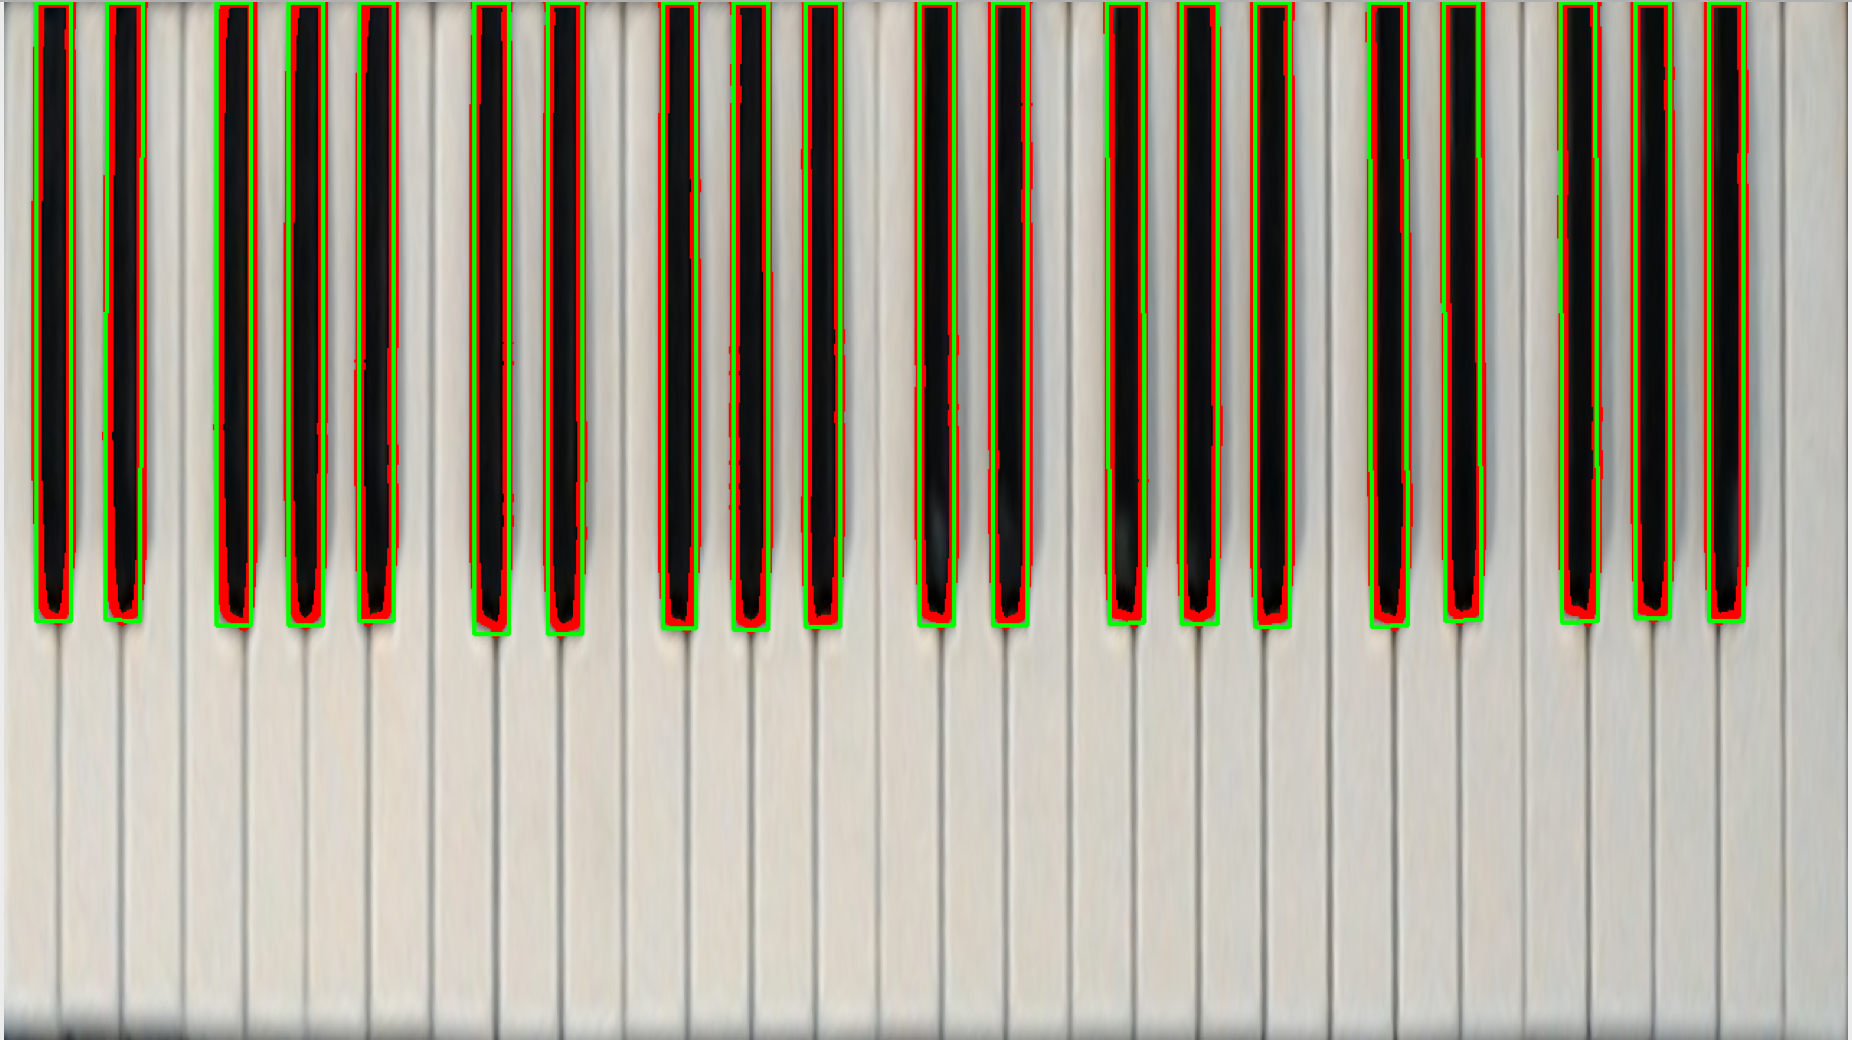
\includegraphics[width=\linewidth]{piano-correction}
    \caption{Homographic correction and key contours}
  \end{subfigure}
  \begin{subfigure}[b]{0.8\linewidth}
    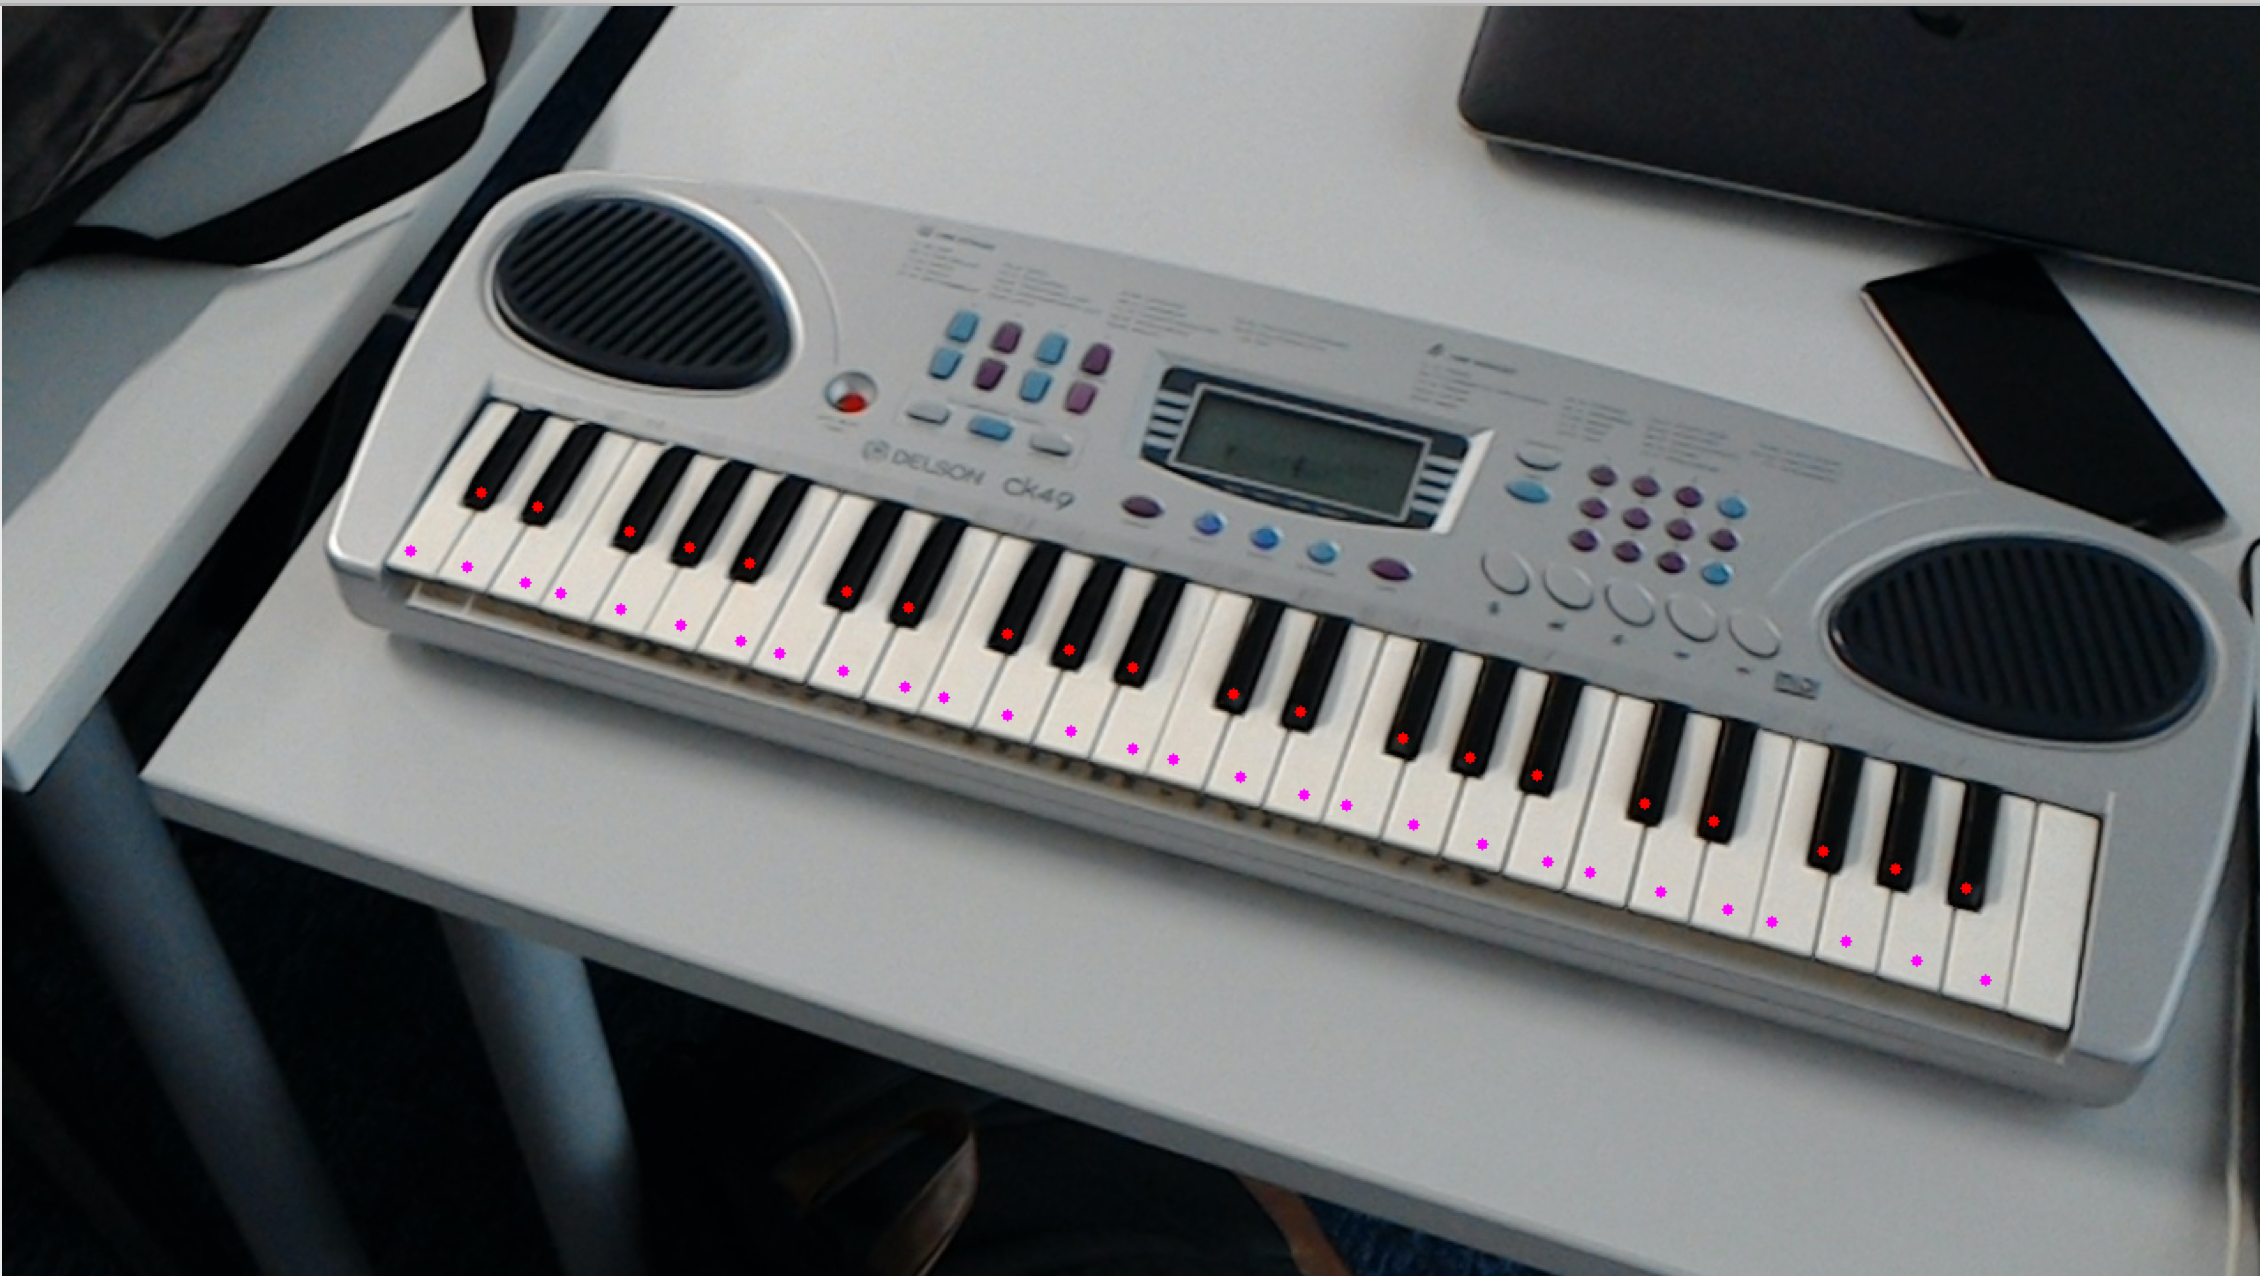
\includegraphics[width=\linewidth]{piano-points}
    \caption{Final result}
  \end{subfigure}
  \caption{Steps for detecting the piano keys}
  \label{fig:coffee3}
\end{figure}

\begin{figure}[H]
  \centering
  \begin{subfigure}[b]{0.4\linewidth}
    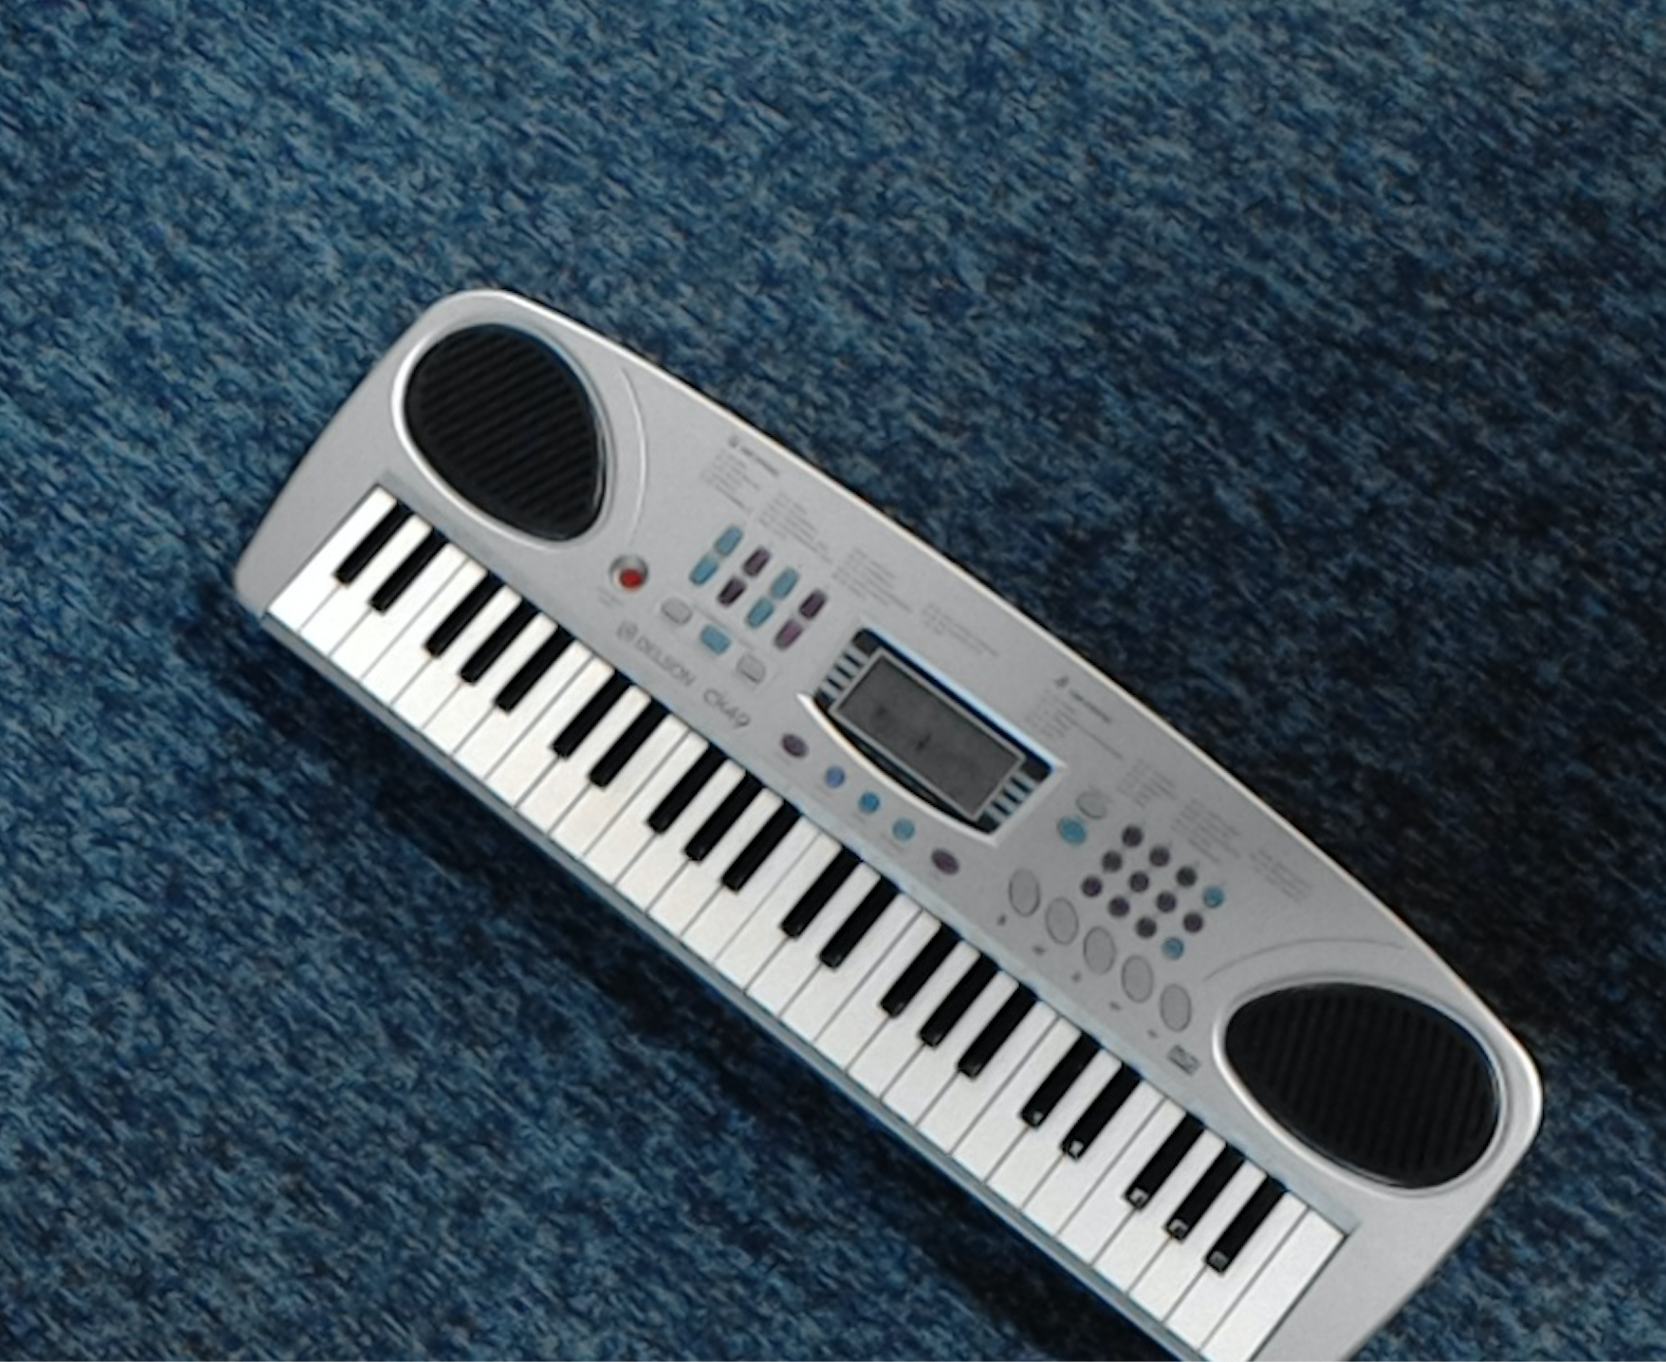
\includegraphics[width=\linewidth]{piano-originalv2}
     \caption{Original Image}
  \end{subfigure}
  \begin{subfigure}[b]{0.577\linewidth}
    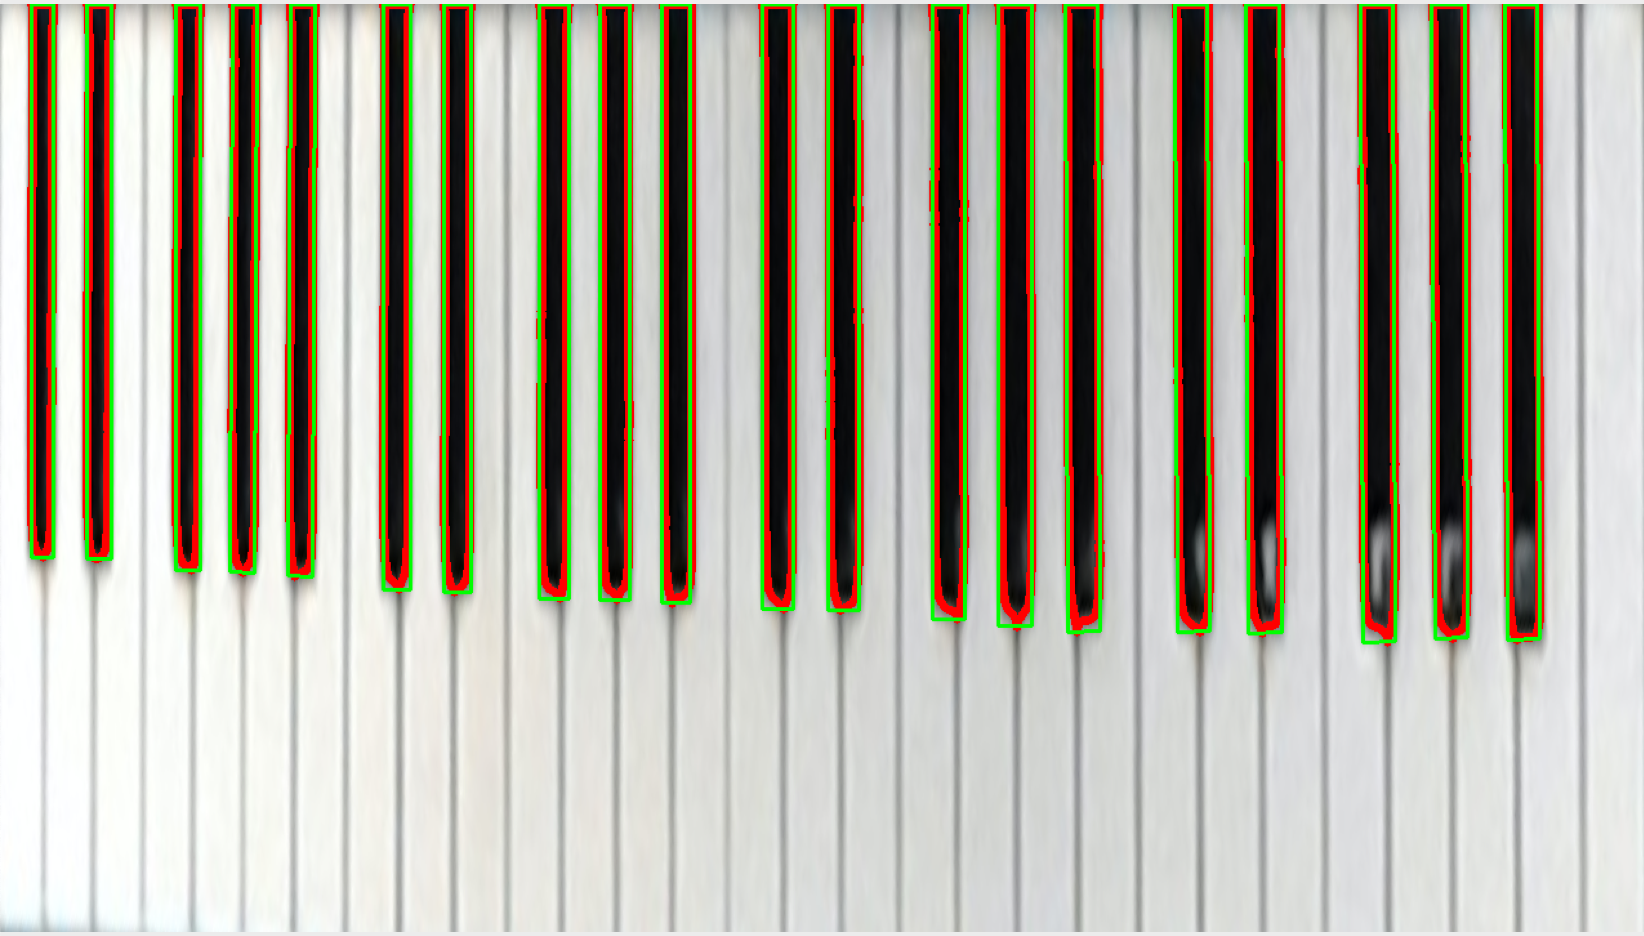
\includegraphics[width=\linewidth]{piano-correctionv2}
    \caption{Homographic correction and key contours}
  \end{subfigure}
  \begin{subfigure}[b]{0.7\linewidth}
    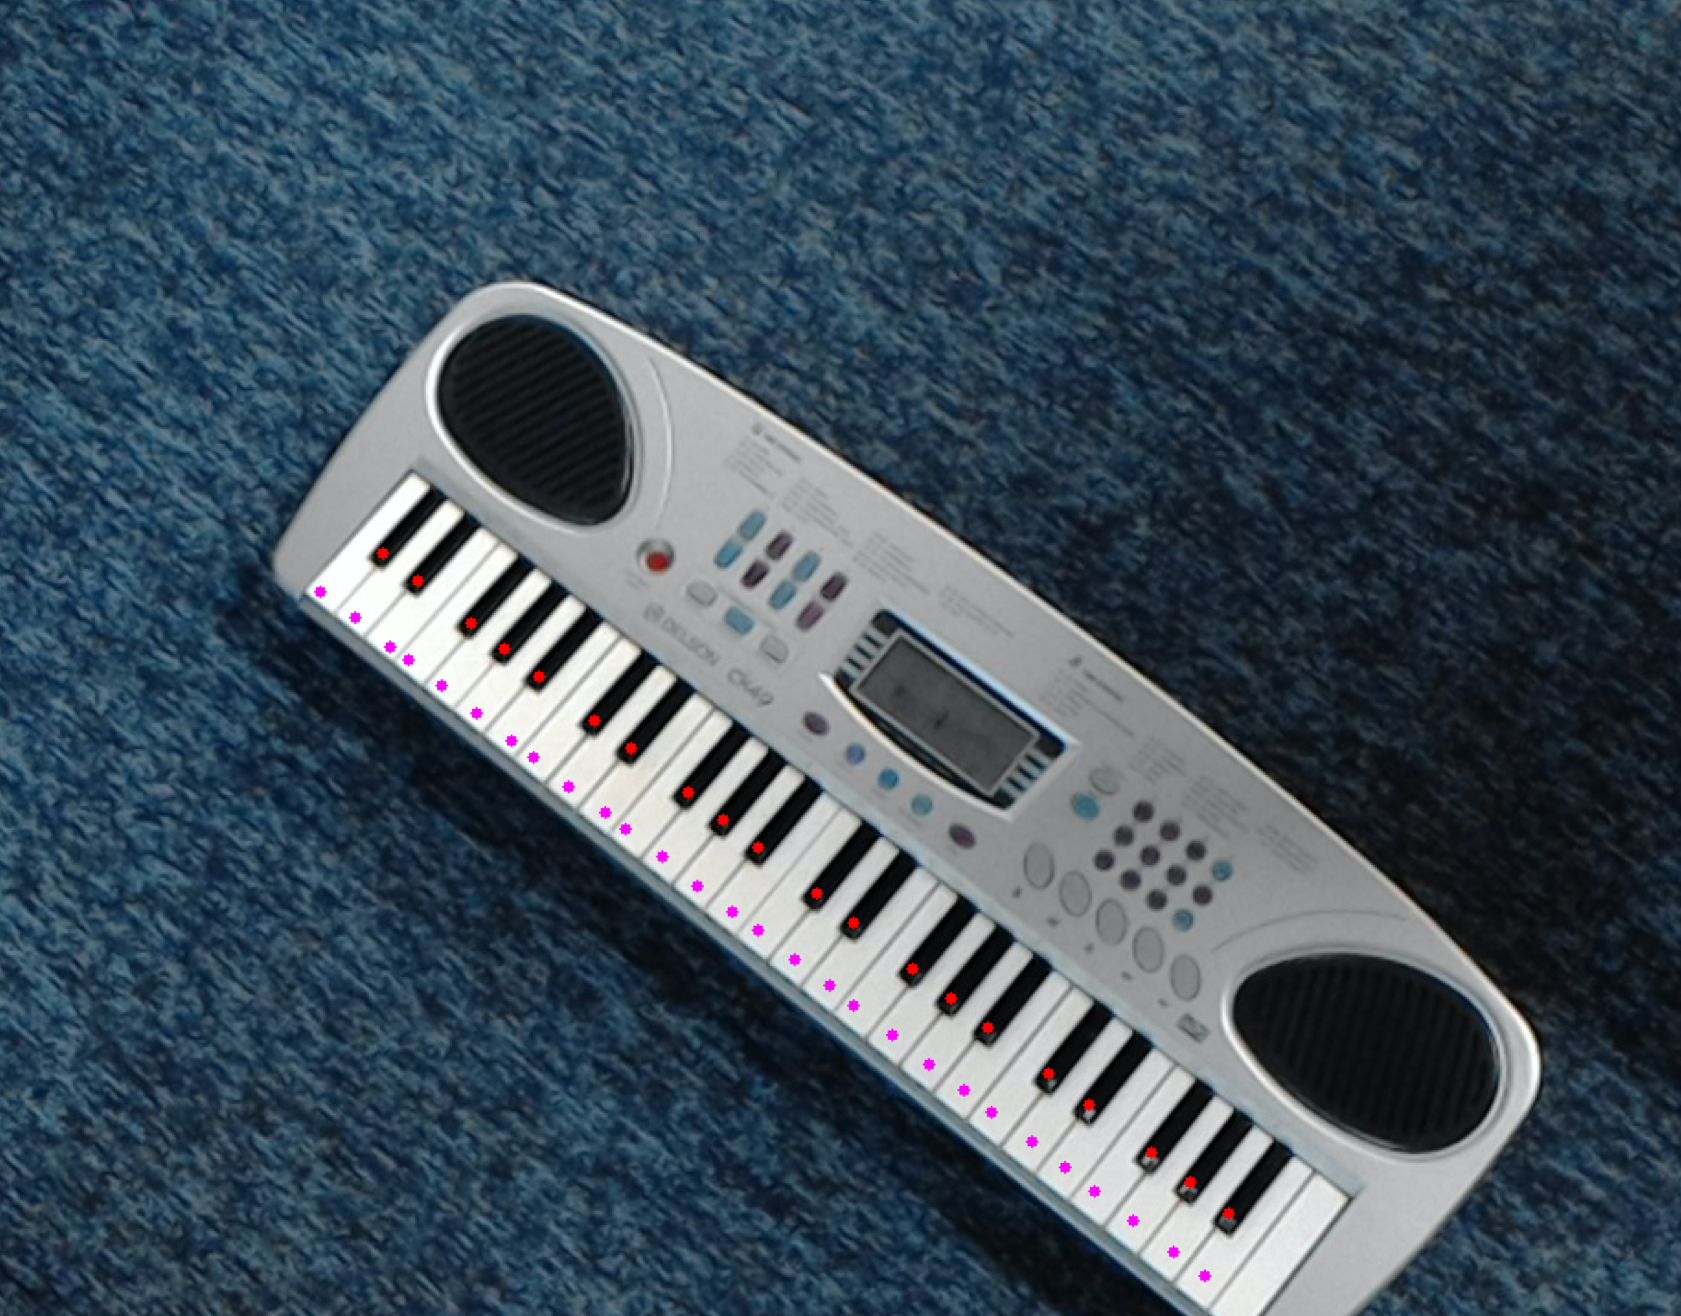
\includegraphics[width=\linewidth]{piano-pointsv2}
    \caption{Final result}
  \end{subfigure}
  \caption{Steps for detecting the piano keys}
  \label{fig:coffee3}
\end{figure}

After receiving 4 coordinates and a picture, using Homogrophic Correction, the image is rotated such that all piano keys have a vertical angle. Then, using a watershed algorithm the contours of all the keys are generated and what is left is to filter the out-layers and to give each contour the musical note that it represents. 

\section{Limitations of the device}

Unfortunately, after we have put together all the parts, we realised that the device we were using (HoloLens) is not powerful enough to maintain the holograms exactly on the position we are spawning them on, thus the holograms were drifting randomly over other piano keys, rendering the experience unusable.

The key component of our approach was the experience given by smart glasses, as other type of AR, like the one given by Handheld devices still represents an unfeasible approach, as we do not want to place a phone or a tablet between the user and the piano.

We believe that in the near future, as the hardware and software are continuously improving (at the moment of writing Microsoft announced a new version of HoloLens that is going to come with built in AI capabilities and improve precision), this approach is going to be realisable.

\section{Alternative approach}
A more analog, but working path that we took is to replace HoloLens glasses with a strip of very small, individually controllable leds that are going to be sticked above the piano keys, one or two leds (depending on their size) are going to directly map one piano key. 

A few seconds before the user would need to press a piano key, the specific leds are going to be lit up, increasing in intensity until the moment they actually need to be pressed, then they will continue to blink prior to other keys needing to be pressed.

If by placing a camera above the piano, using image processing we could detect if the required piano keys were actually pushed correctly and offer specialised lightning feedback and dynamic context advance of the song progress.

For this approach, the strip of leds was connected to an Arduino board which exposes an API through that all the leds can individually be controlled. A Raspberry PI was used also used to orchestrate all the components.

One disadvantage of this approach is given by the variable number of keys a piano has and the variation in width that can occur (for each key in particular and for the gap between two keys), giving the need of calibration prior of permanently positioning the leds .

\section{Conclusion}
This generation of augmented reality enabled devices are not powerful enough to sustain such an use case, moreover at the current time these devices are in early stages, mainly targeting researchers and developers, their price making them unreasonable for the average individual. Fortunately, the progress towards newer iterations that will come with improved precision, performance and a better prices are soon to be released, rendering this approach valid.

From the point of view of bringing additional educational value, they truly have the potential to render the already available information on ways that could not be done before, thus being able to surpass even the classical in-class experience, even removing the limit of physically needing to be at a certain  time and location to benefit from such activity.
\begin{figure}[]
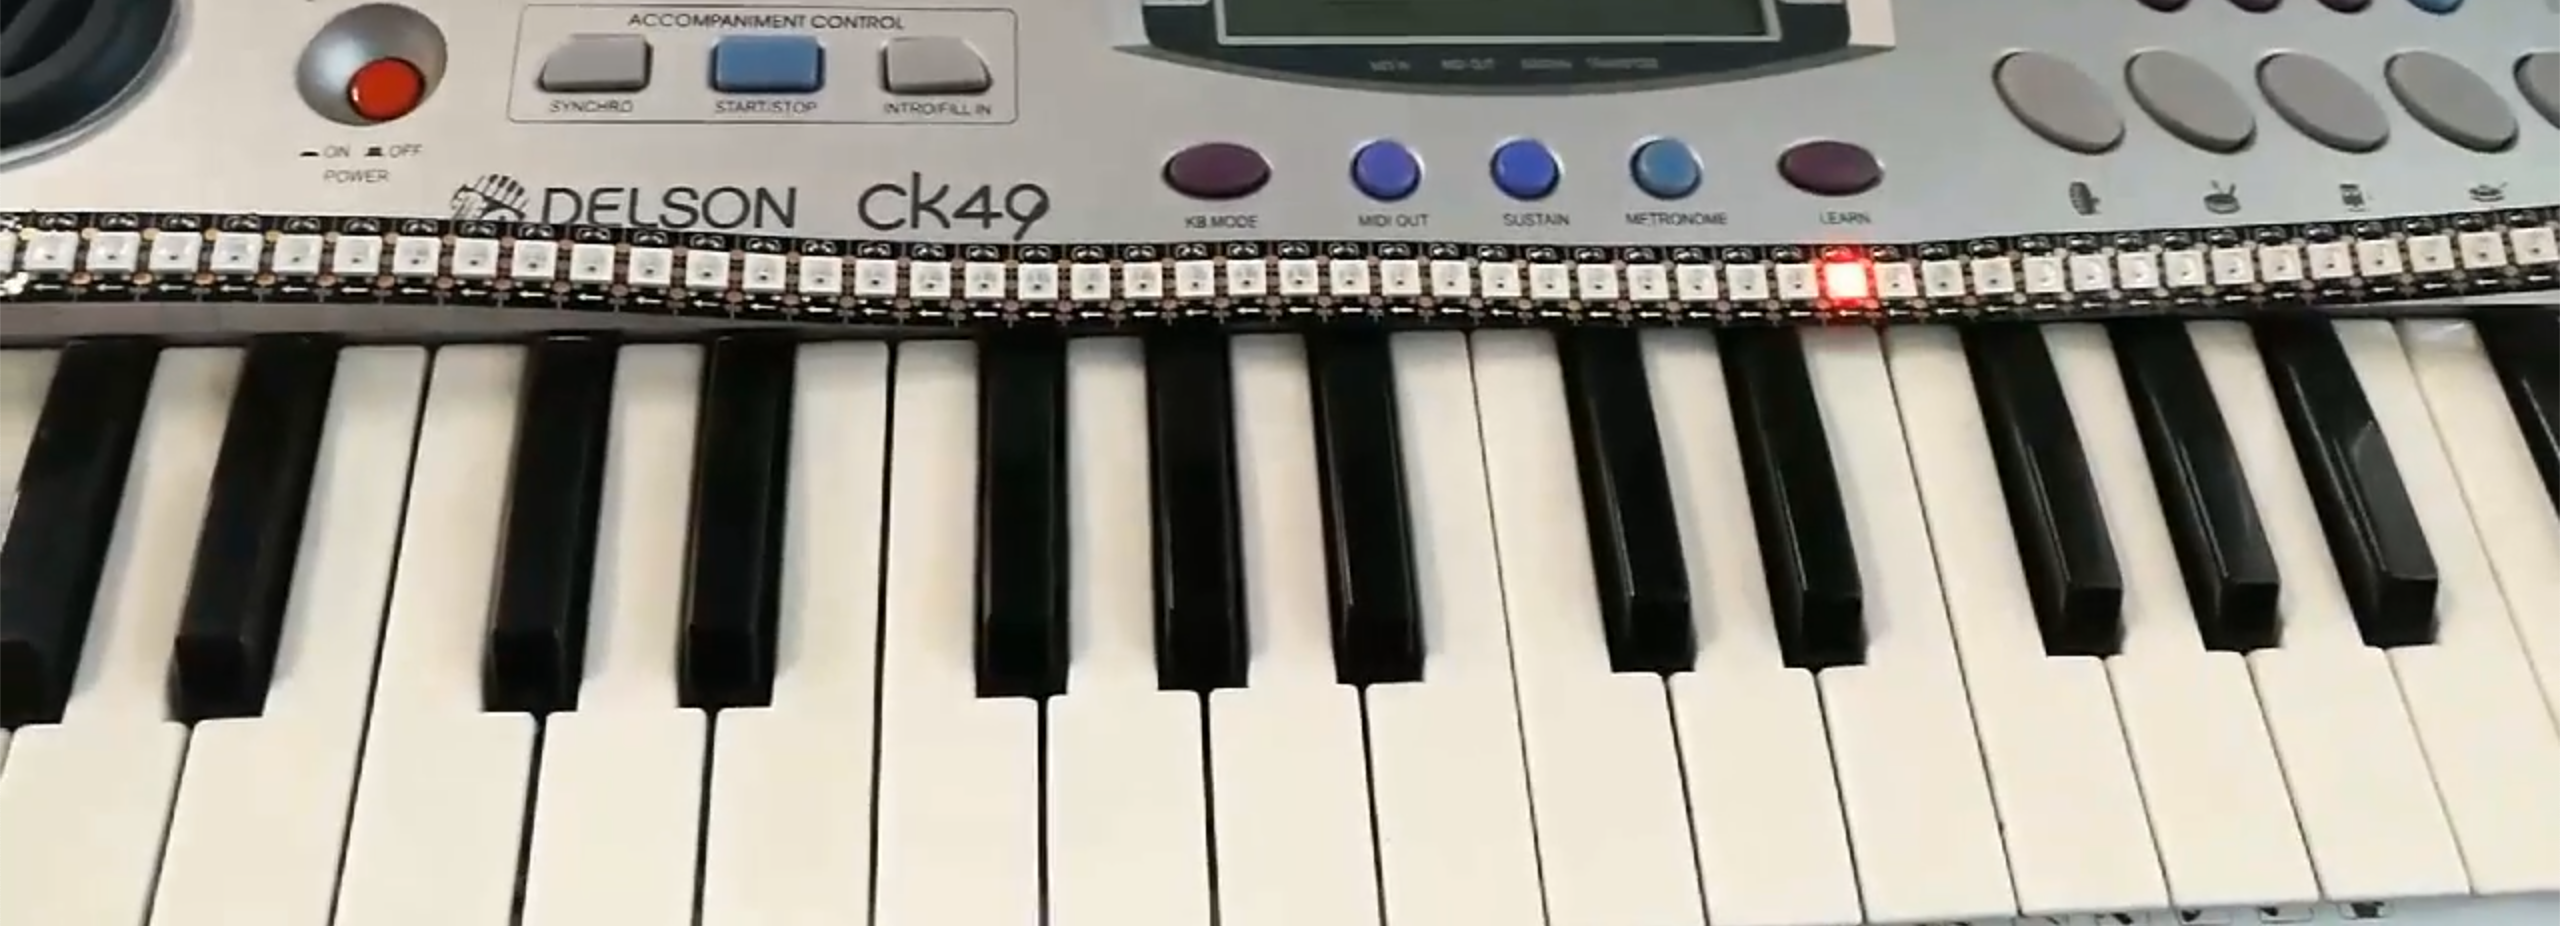
\includegraphics[width=1.0\textwidth]{piano-leds}
\centering
\label{fig:feature-points}
\caption{Strip of leds sticked to the piano}
\end{figure}


\chapter{Application in Computer science}

\section{Problem}
As Computer Science is a field that is dramatically increasing in popularity and still not quite keeping yet with the demand, forming a way of thinking suitable for a programmer takes time and practice, but by starting at a younger age, when the mind is at it peaks in terms of forming and grasping new knowledge, the chances to be successful in this domain will drastically improve.


\section{Related work}
These kinds of applications are already known for their efficiency, Hour of Code is one of the most popular platforms and movements (that hosts and encourages the apparition of code tutorials in this format), becoming a global success with over 2 million students and a total of 750 millions hours of coding. Its success is standing on gamifying the process of coding into a puzzle-solving activity that attracts people of all ages (from 5-year-old kids with animated levels to young adults). The goal of the project is to expose as many individuals as possible to one hour of code, amount that is enough to form a spark that can lead to a lifelong passion.

The coding  activities are usually found in a web or mobile format, making them easily accessible to the most used devices like laptops, mobile phones and tablets.

\section{Solution}
Using an IPad, ARKit, and ScratchBlocks we have developed a solution called ArRobotCode that uses Augmented Reality to aid in grasping the basic knowledge needed for writing algorithms, everything being packed into a form that tries to be more tightly coupled with the reality, making concepts that are very abstract for kids of that age understandable.

The lessons are presented in a level format (a multitude of levels organised by complexity and topic) in which his or her role is to fly a spaceship from Earth to Moon. This can be done by providing a list of instructions so that the spaceship follows a given route (and does not deviate).

We believe that by taking the already proved success of other similar initiatives (like the one presented above) and adding all the benefits that come with augmented reality, will render a superior experience that will catch and be able to maintain the attention of a younger audience for longer periods of time.

\section{ScratchBlocks instructions}
\begin{figure}[H]
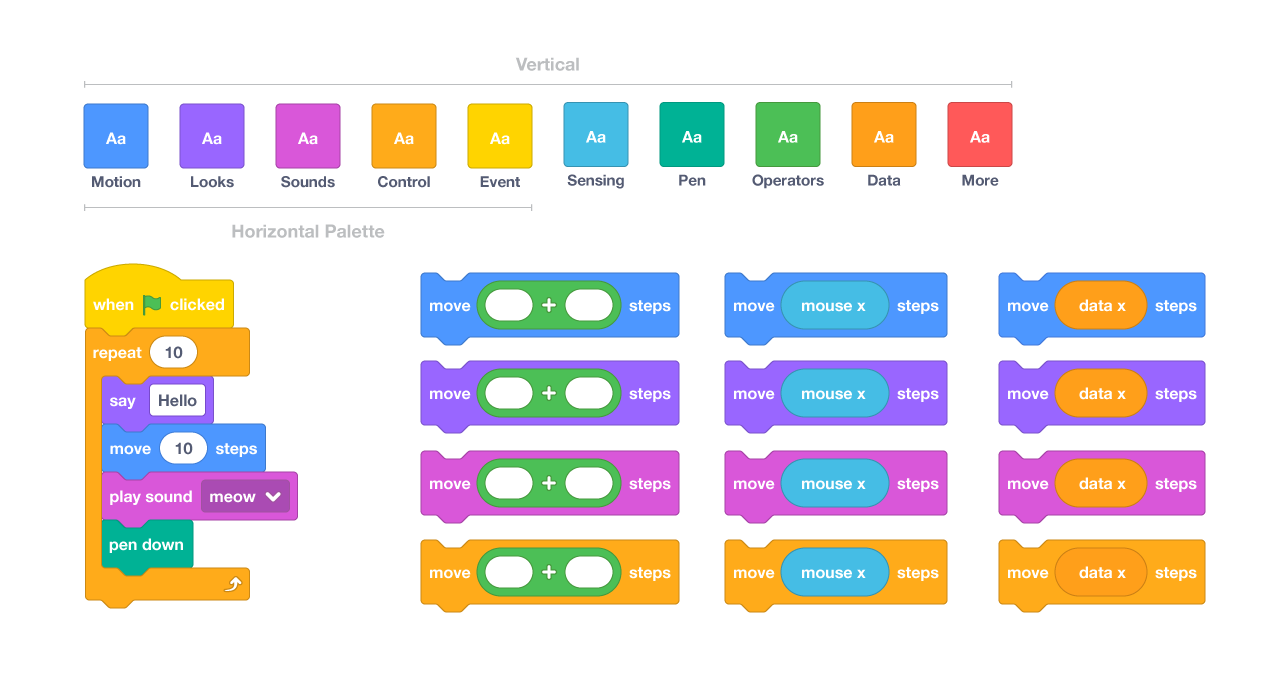
\includegraphics[width=1.0\textwidth]{scratchblocks-2}
\centering
\label{fig:hololens}
\caption{Scratchblocks}
\end{figure}

Scratch Blocks is a fork of Google's Blockly project that provides a design specification and codebase for building creative computing interfaces dedicated to young children. Together with the Scratch Virtual Machine (VM) this codebase allows for the rapid design and development of visual programming interfaces. Unlike Blockly, Scratch Blocks does not use code generators, but rather leverages the Scratch Virtual Machine to create highly dynamic, interactive programming environments.

\begin{figure}[H]
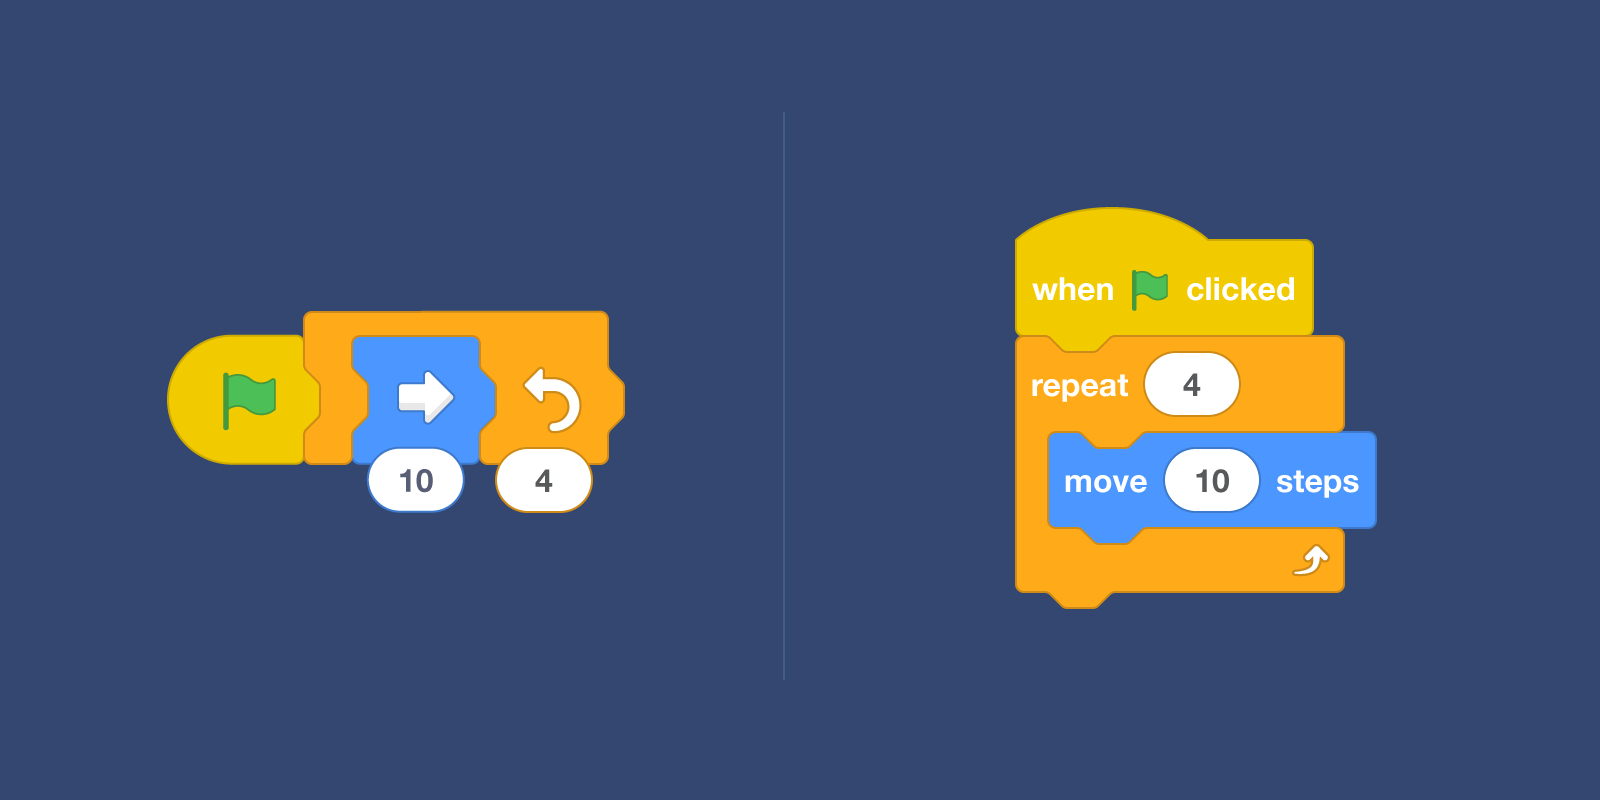
\includegraphics[width=1.0\textwidth]{scratchblocks}
\centering
\label{fig:hololens}
\caption{Scratchblocks}
\end{figure}

There are two types of blocks, horizontal and vertical ones. The horizontal blocks provides a simpler UI, focused on visual indications instead of textual ones, the downside being that it is fairly limited. The second category will be more familiar for those which have coded before, it allows for a more powerful set of instructions and more customisation, this being the reason behind why it was chosen for this application.

\begin{figure}[H]
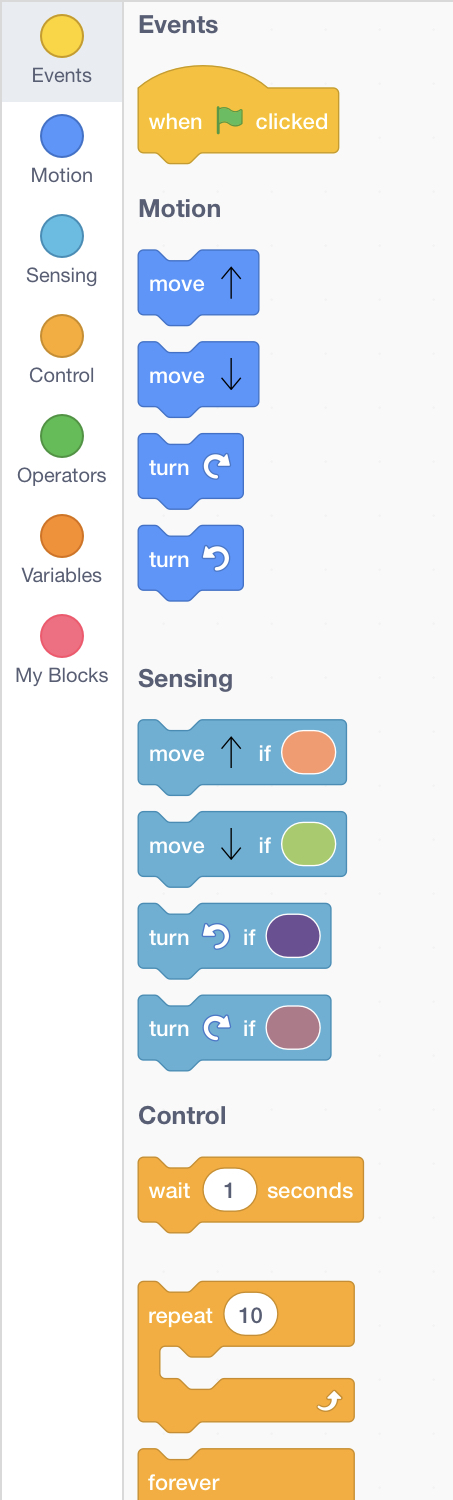
\includegraphics[width=0.4\textwidth]{allInstructions}
\centering
\label{fig:hololens}
\caption{Instructions used in ArRobotCode}
\end{figure}

For the purpose of this project the instructions have been refined to be powerful enough but suited for the age group that is targeted. There have been kept only a subset of all the available instructions and categories, also they have been updated to a contain more visual information. 

\begin{figure}[H]
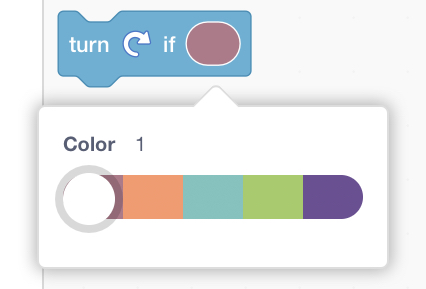
\includegraphics[width=0.4\textwidth]{newIf}
\centering
\label{fig:hololens}
\caption{Inline conditional instructions}
\end{figure}

Inline conditional move instructions have been created to strip town the classical 'if'  to be more digestible for the youngest, basically it allows the spaceship to move or rotate towards a direction depending on the color  of the tile that the spaceship is sitting on.
\section{Architecture}

\subsection*{Main Activity}
\begin{figure}[H]
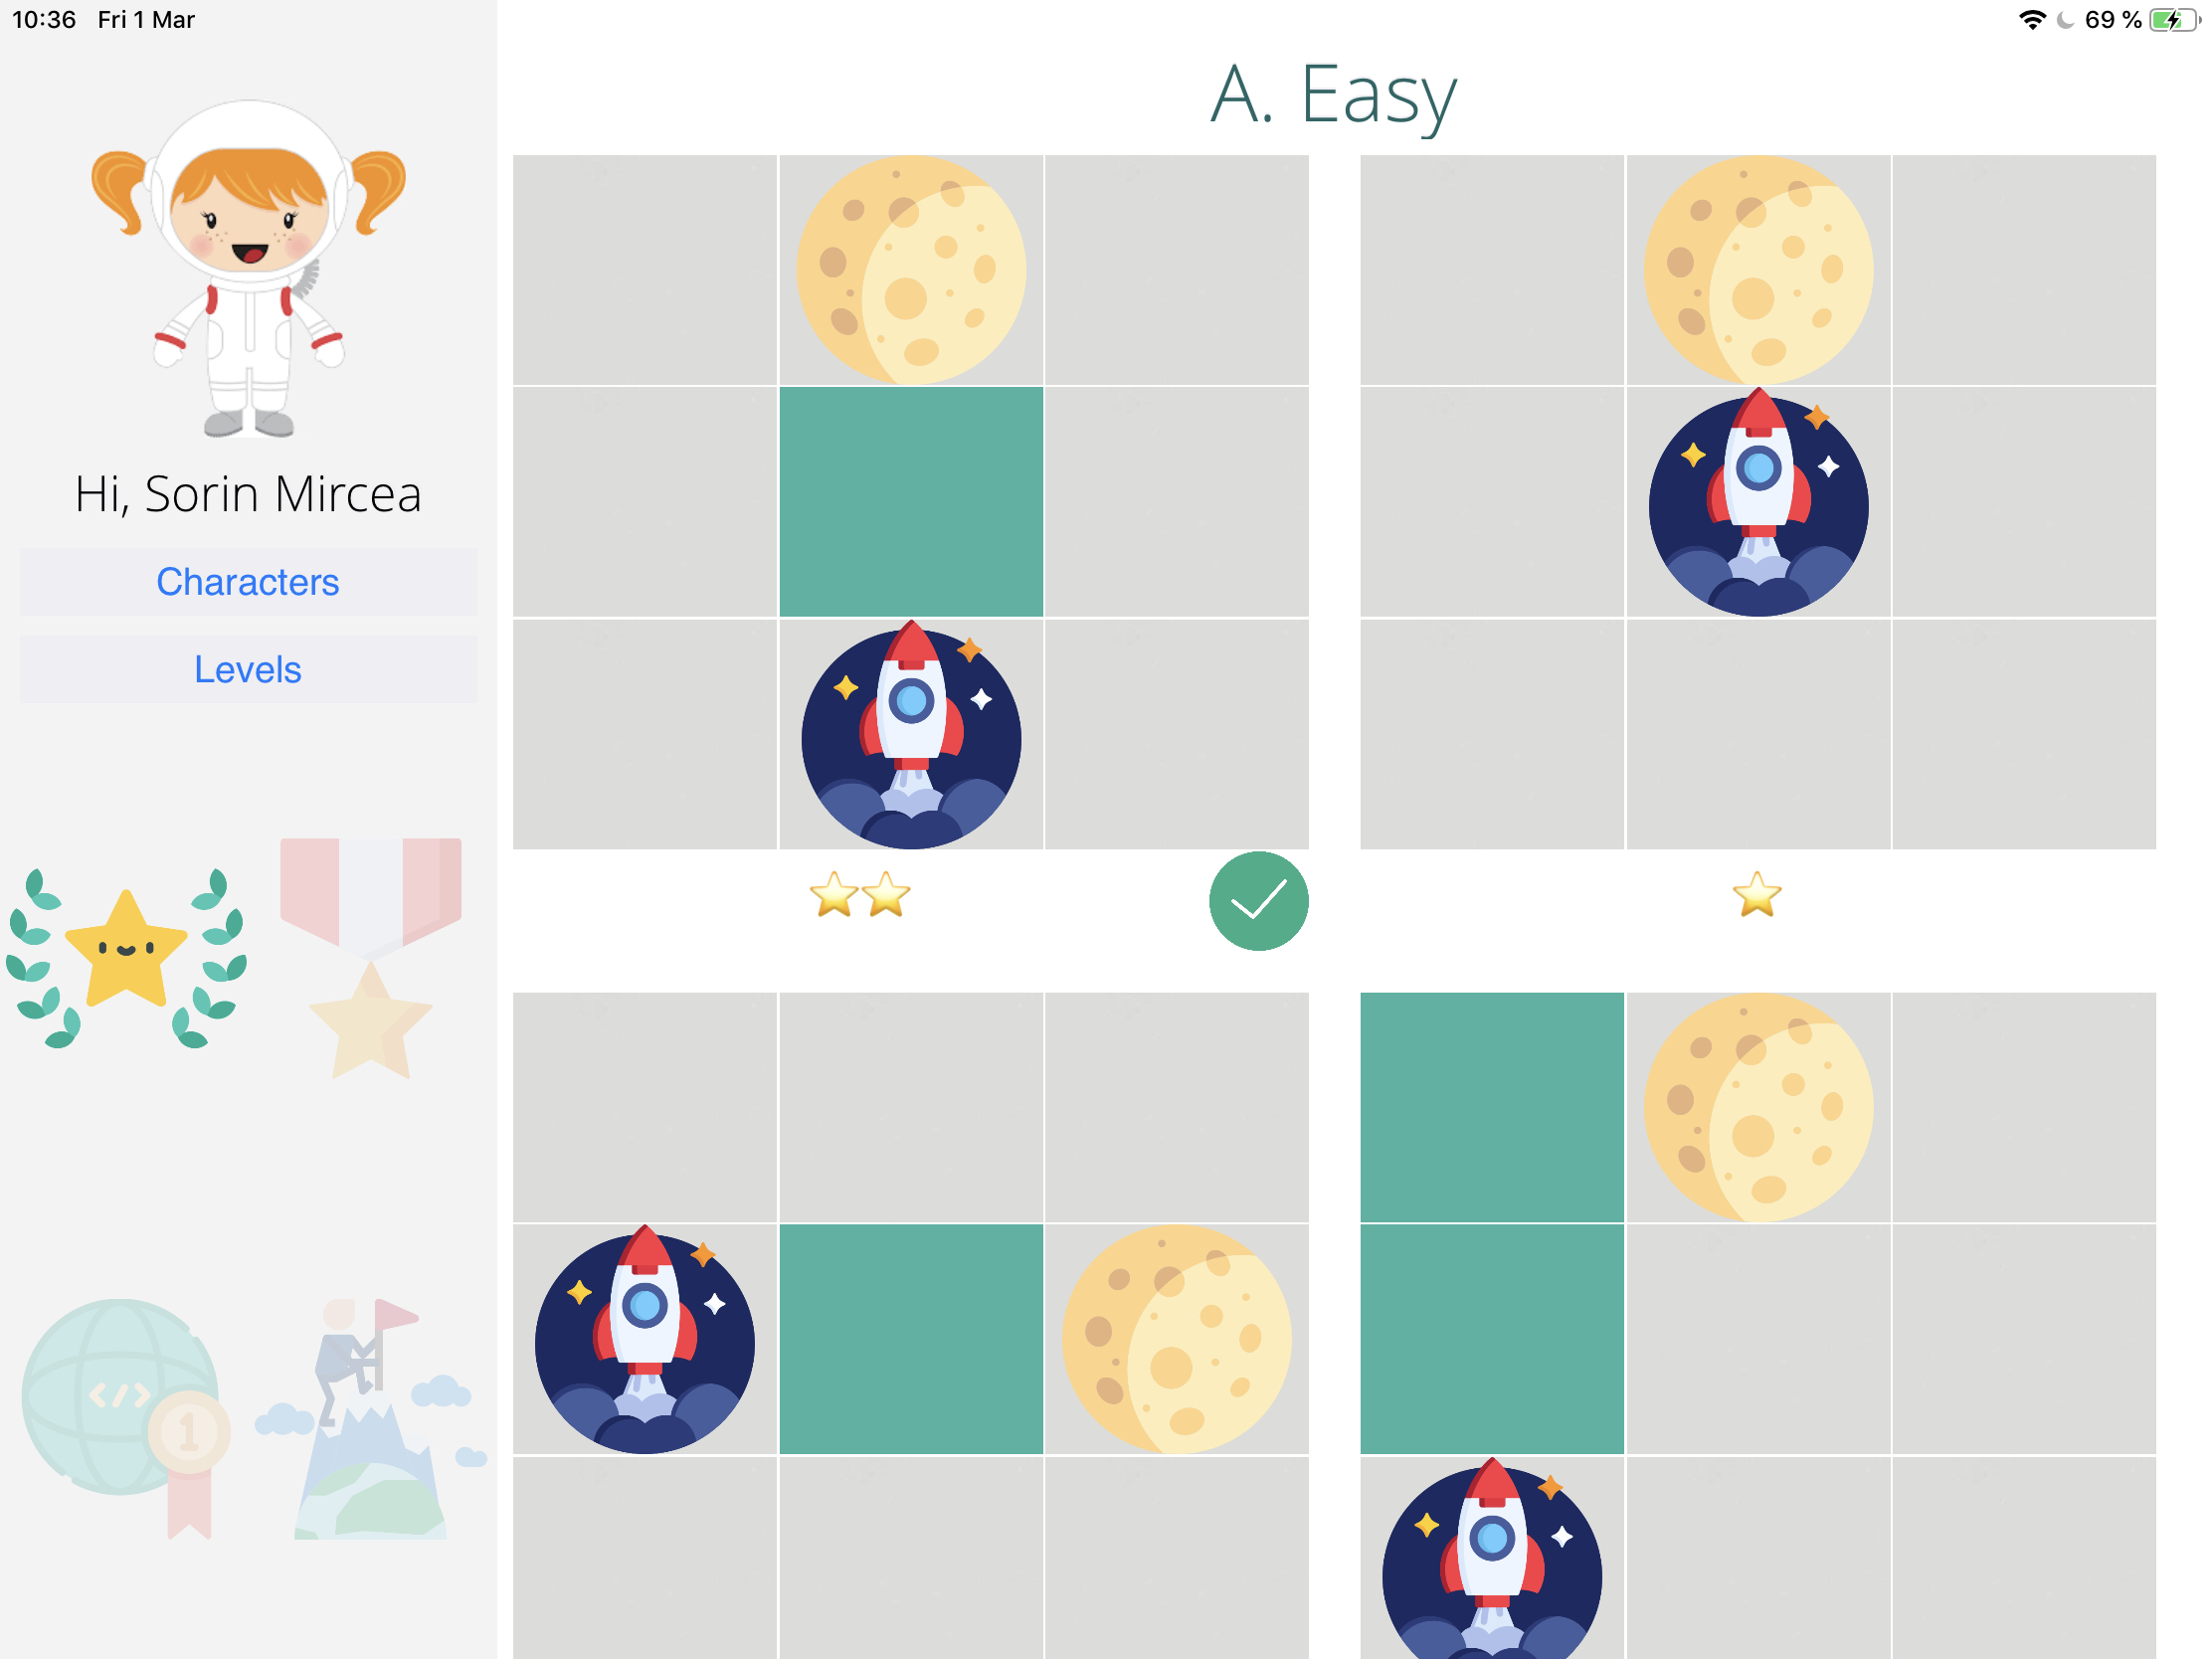
\includegraphics[width=1.0\textwidth]{ArRobotCode0}
\centering
\label{fig:hololens}
\caption{Scratchblocks}
\end{figure}

The home screen of the applications consists of a list of the levels organised by difficulty. All the completed levels are marked accordingly with a green tick to stimulate the feeling of accomplishment. 

The levels are organised in chapters based on their difficulty and on different algorithmics aspects that they emphasise. The content can be dynamically changed directly from the application by anybody that has administrative privileges, and it will propagate to all other users without the need to launch a separate update.

\subsection*{Game Activity}
\begin{figure}[H]
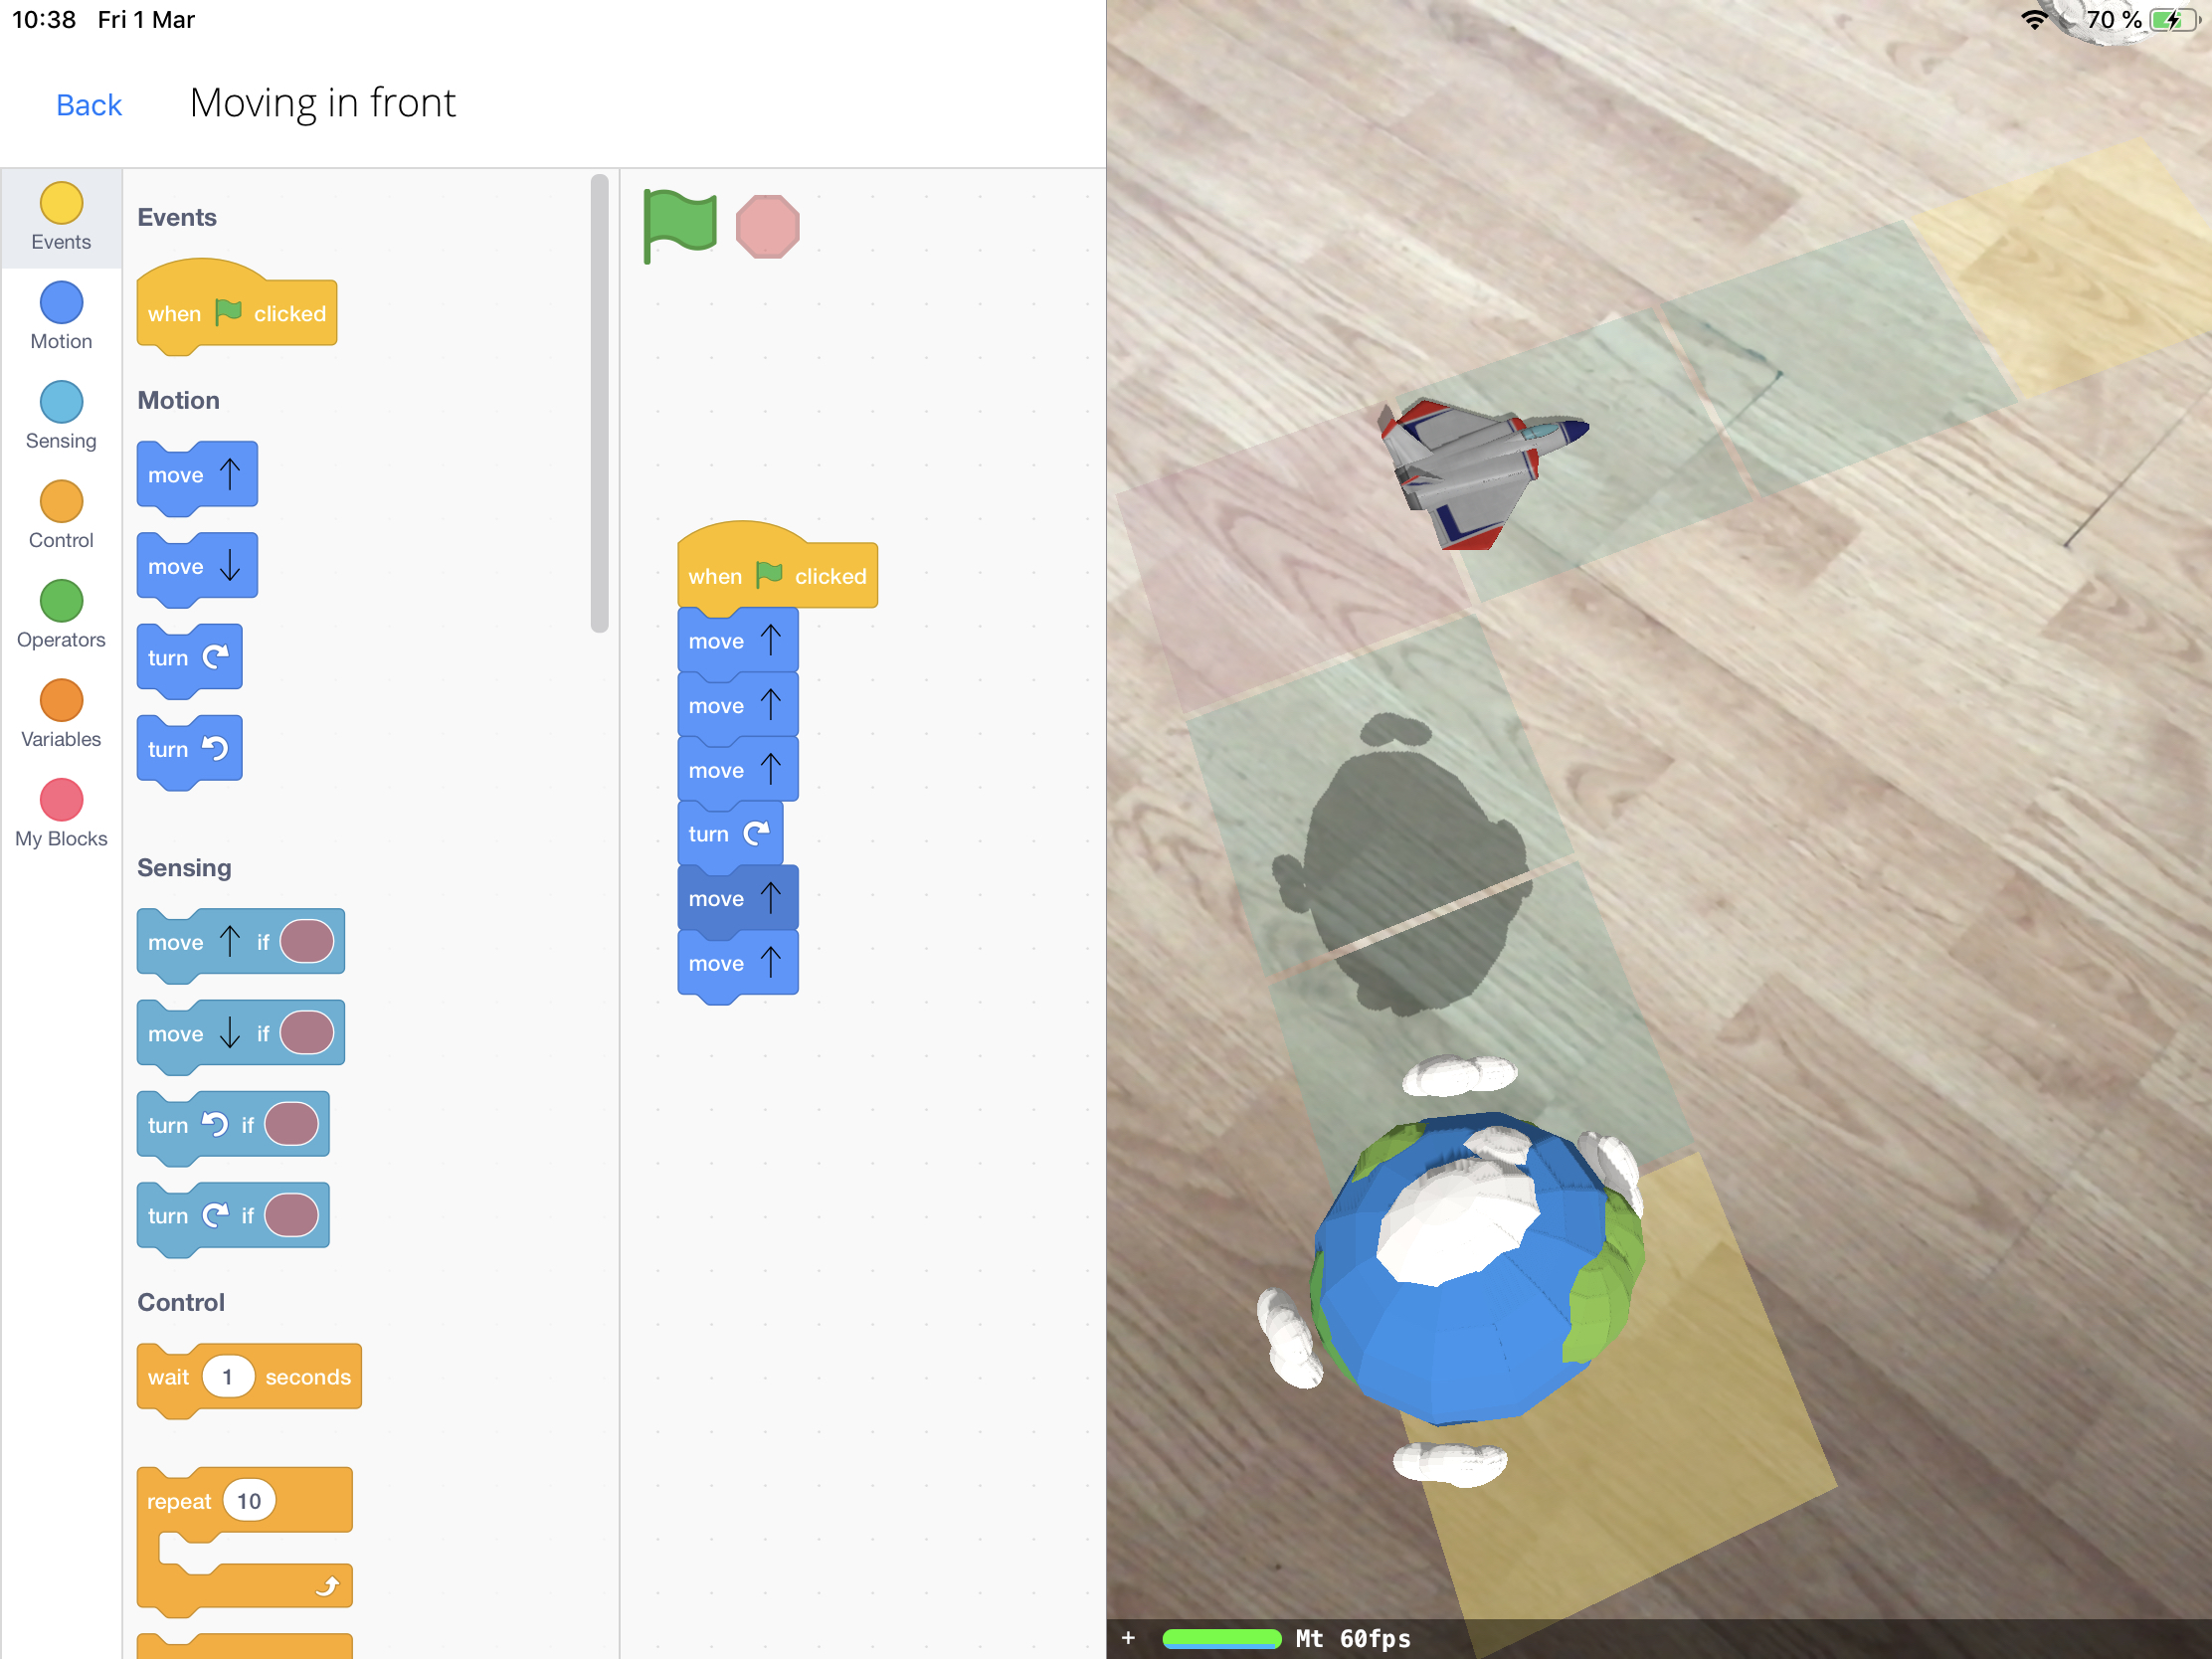
\includegraphics[width=1.0\textwidth]{ArRobotCode2}
\centering
\label{fig:hololens}
\caption{Scratchblocks}
\end{figure}
The game screen is split into two parts. The one from the left is a WebView that hosts a heavily modified version of ScratchBlock, and the right part consists of the Augmented Reality view that renders the game scene over the reality. There is a bridge that allows permanent bi-directional communication between the two parties.

When the run button is pressed to execute a sequence of instructions an event is sent to the WebView signalling to trigger the compilation of the code, thus forming a sequential list with all the instructions needed to be executed (if there is a forever instruction, the output will be of course truncated). When this list reaches the native section, the spaceship is moved to the initial position of the board, and each sequence is executed one by one (only one per second, to allow the user to observe every action and the exact moment an eventual mistake occurs). Before starting the movement animation of the spaceship, the native part sends an event to ScratchBlocks specifying witch instruction block is going to run, so that it glows, emphasising it.

Horizontal plane detection is a builtin feature of ArKit and it is used right after a level was loaded, more exactly when the application is entering in a state where it searches for suitable places to render the scene on. At that moment, by taping on one of them, the user can select the plane where the actual game scene is going to be instantiated. Due to the fact that the plans dimensions are variable (it can be spawned on a large floor or on a tight table), the scene scales accordingly. This process happens every time a new level is loaded, to enable for new location to be found and chosen.
\subsection*{Level Builder}
\begin{figure}[H]
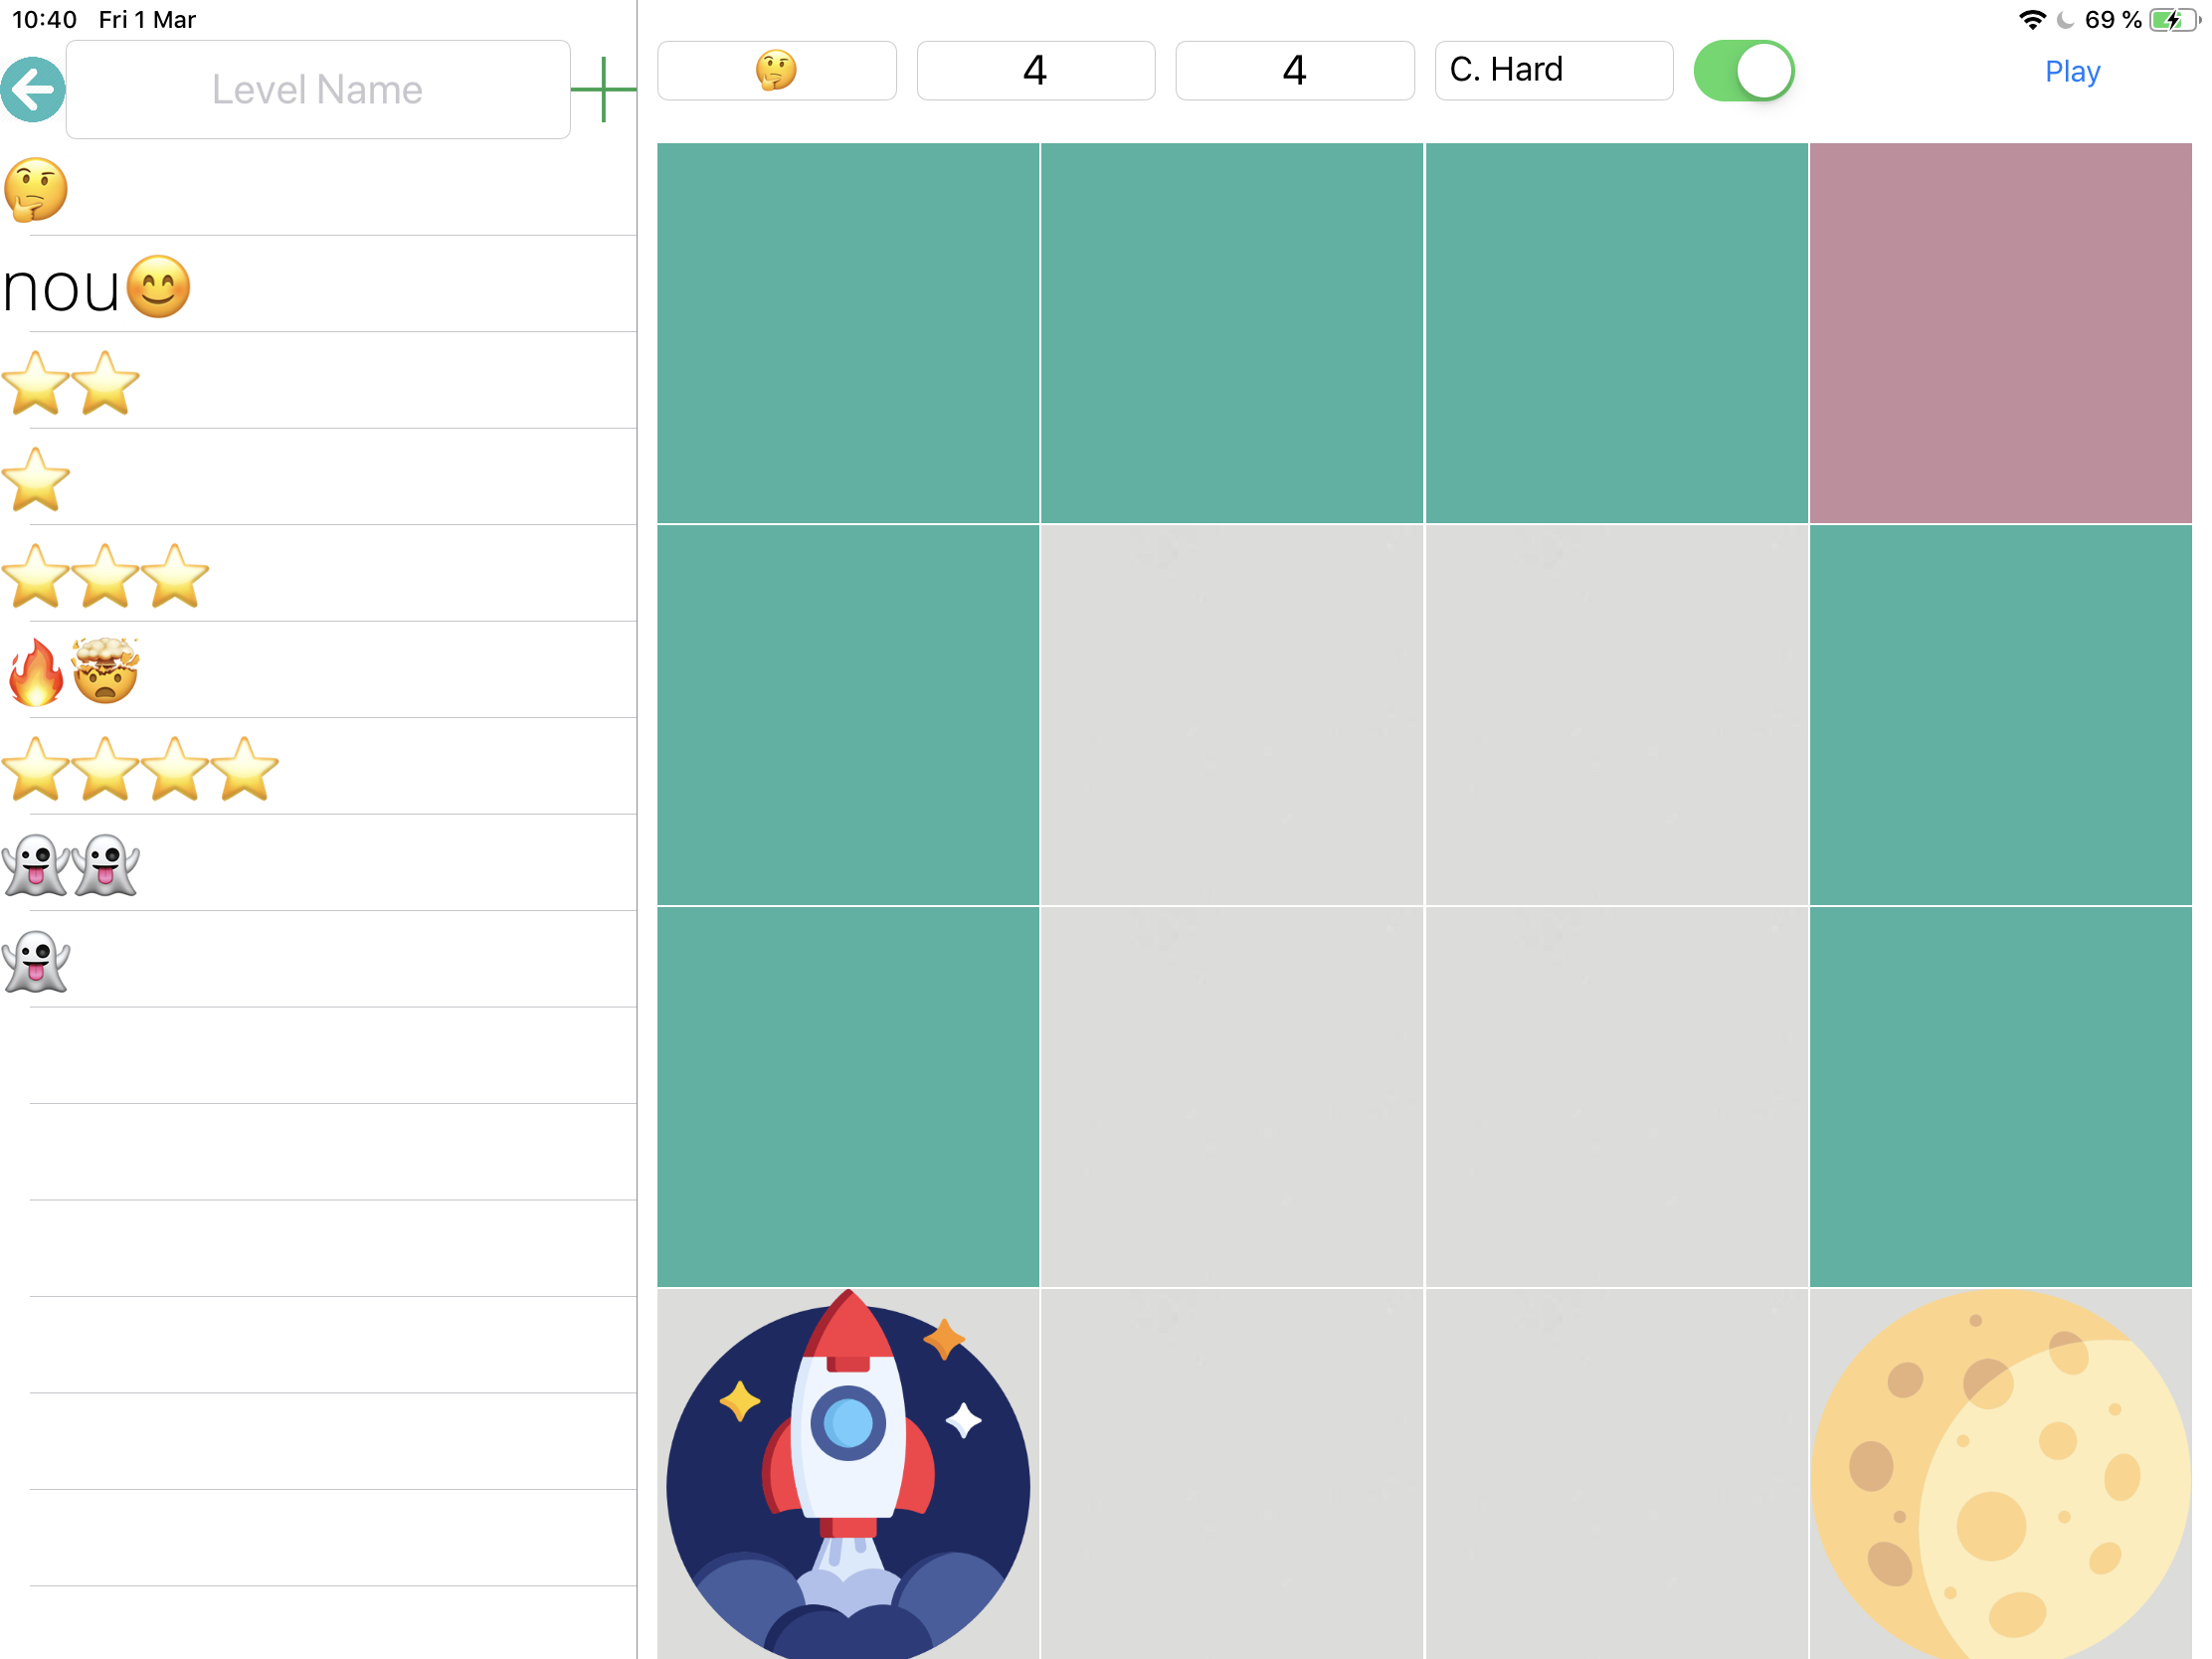
\includegraphics[width=1.0\textwidth]{ArRobotCode3}
\centering
\label{fig:levelBuilder}
\caption{Level builder interface}
\end{figure}

One of the most important features is the in-game level builder that allows users to create and experiment with their own levels, providing a signifiant boost in creativity and understanding. 

Tiles are of the following types:
\begin{enumerate}
\item Start position - Spaceship
\item End position - Moon
\item Free
\item Occupied
\begin{enumerate}
\item Pink
\item Orange
\item Blue
\item Green
\item Purple
\end{enumerate}
\end{enumerate}

In order to interact with User Interface in the building menu, one has to use a few predefined gestures, a simple tap would switch between a free tile and a default green occupied one. By swiping right or left on an occupied tile, one can cycle between the five different available colours. In order to trigger the starting position, a long tap is required and from this current state if tapping one more time the end tile will appear, and after one more tap it will reset back to being a free cell.

The grid size is also customisable, the number of rows and columns can be changed from the inputs that are situated on top of the screen. 

If the account has administrative privileges, like in figure \ref{fig:levelBuilder} two extra inputs are going to be visible, a text field that contains the name of the category that the level is going to have and a toggle to publish it. 

There is also the possibility to test the levels while building them by using the dedicated button.
\subsection*{Data Persistence}
Cloud Firestore (from FireBase) is used as the persistence layer, it is a scalable NoSQL cloud-hosted database with offline mode and syncing capabilities.

It supports flexible, hierarchical data structure, files being organised in documents (the equivalent of tables from SQL) that further split into collections. It features realtime support, callbacks that are triggered if a substructure of the registered node is updated. Even if the application is in an offline state, all the data changes are going to be cached and then synced when the device comes back online. It also enable authenticaation integration with 3rd party services, in ArCode the option for one-click Google login is used, no other data being requested from the user.

For the purpose of this project the data is divided into four collections:
\begin{enumerate}
\item Users: beside basic user information like the token, role, it contains the currently selected character and a reference to all the completed achievements and levels
\item Levels: name, chapter name, height, width, reference to the user that created it, boolean specifying if the level is public or not and a sub-list of width*height length containing the type of tile
\item Characters: name of the character, icon and the number of completed levels required for unlocking it
\item Achievements: name of the achievement, a short description and its picture
\end{enumerate}

\subsection*{Reactive Programming}

\begin{figure}[H]
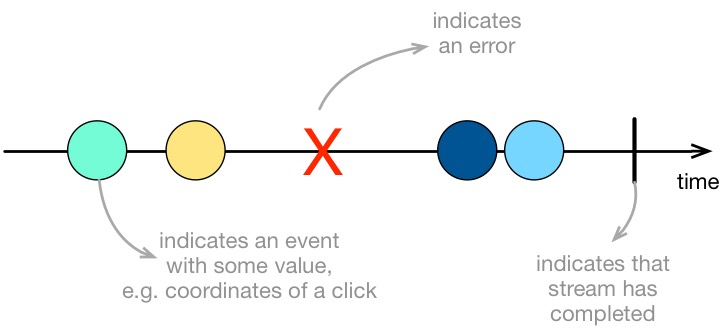
\includegraphics[width=0.6\textwidth]{streams}
\centering
\label{fig:reactive-pgrogramming}
\caption{Example of reactive programming }
\end{figure}

Represents programming with asynchronous data streams. Its functional part is what it makes it an truly elegant way of writing code. Streams are cheap, ubiquitous and basically anything can be a stream: variables, user input, properties, data structures, etc. A stream can be used as an input to other stream, it can be merge into two streams, filtered to get only the events that impose interest, mapped to other  values and so on.

\begin{figure}[H]
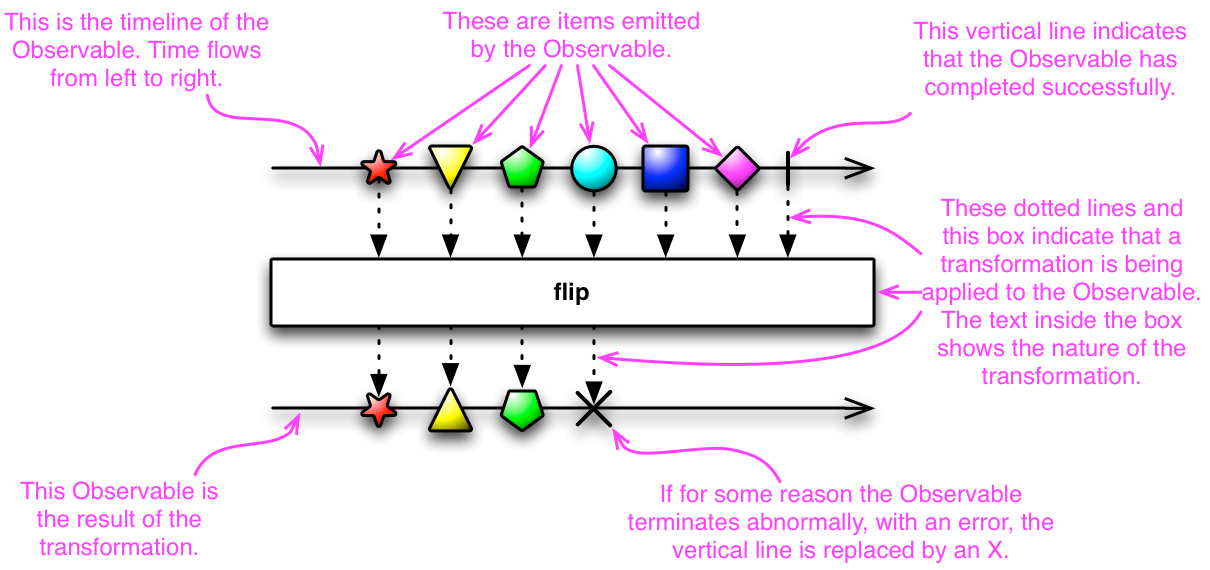
\includegraphics[width=1.0\textwidth]{observable-doc}
\centering
\label{fig:feature-points}
\caption{ \cite{reactivexDocumentation} }
\end{figure}


An observer subscribes to an Observable making it react to whatever item or sequence of items the Observable emits. Concurrent operations are facilitated by using this pattern as there is no need to block while waiting for an Observable to emit object.

A subject is a bridge or a proxy that acts both as an observer and as an Observable. Because it is an observer, it can subscribe to one or more observables and because it is an observable it can pass through the items it has observed by reemitting them, it can also emit new items.

There are four varieties of a Subject, all designed for different use cases:
\begin{enumerate}
\item Async Subject: emits only the last value emitted by the source Observable and only after that source Observable completes
\item Behaviour Subject: when an observer subscribes to a BehaviourSubject, it begins by emitting the item most recently emitted by the source Observable
\item Public Subject: it emits to an observer only the items that have been emitted by the source Observable subsequent to the time of subscription
\item Replay Subject: it emits to any observer all the items that were emitted by the source Observable, regardless of when the observer subscribes. Some implementations replay only a specific number of past emitted events.
\end{enumerate}

RxSwift is the implementation of rx that was used extensively throughout this project. Alongside it, RxGesture was used to provide rx capabilities for detecting different gestures like pan, rotation, swipe and so on.

The application contains multiple repositories for levels, users, characters and achievements. Each repository is treated as a single source of truth and data propagation throughout all the views, for this reason each repository is also a singleton. The repositories output an observable allowing different parts of the program to subscribe and watch for any changes. The outputed observable observes an internal Replay Subject having a buffer size of 1, this allows for every component and the subscription time to receive the latest version of the data without needing to wait until new data is emitted.
\begin{figure}[H]
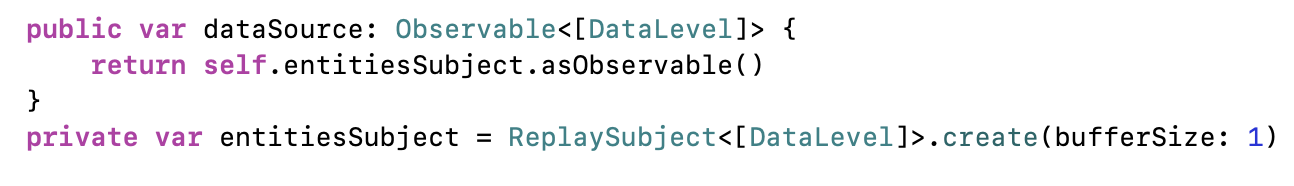
\includegraphics[width=1.0\textwidth]{reactive-repository}
\centering
\label{fig:reactive-repository}
\caption{Repository integration with reactive programming }
\end{figure}

The instructions captured from ScratchBlocks JavaScript virtual machine are enqueued in an Behaviour Subject for the AR rendering controller that takes one instruction per second and executes its. The role of the delay is to provide enough time for the animations to finish rendering. 

One advantage of using reactive programming comes from easily being able to change the thread used for the subscription and observer code (thus leaving the main thread as uncluttered as possible to keep the smoothness of the user interface)
\begin{figure}[H]
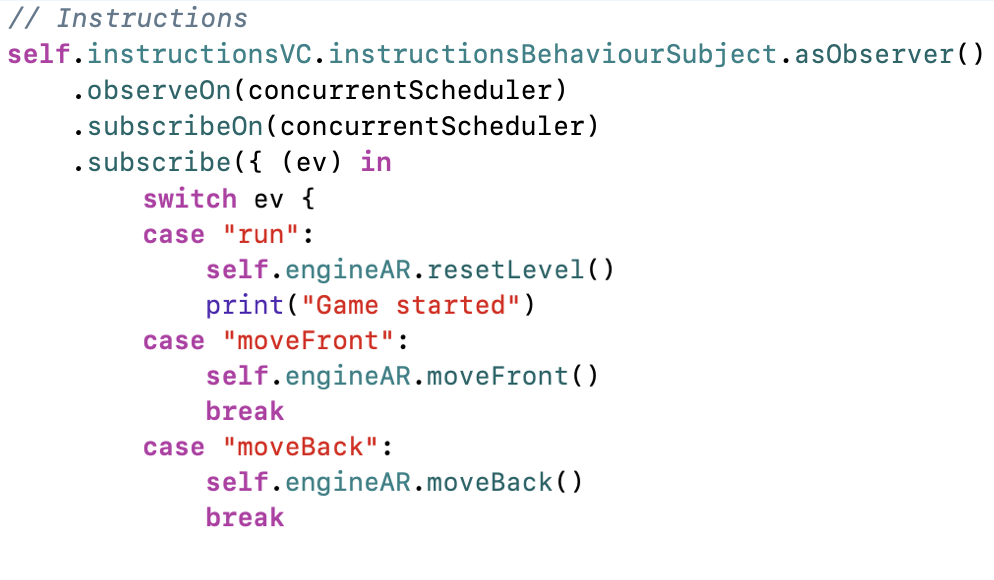
\includegraphics[width=0.8\textwidth]{reactive-instructions}
\centering
\label{fig:reactive-repository}
\caption{Example of reactive programming }
\end{figure}

Model-view-viewmodel pattern, along reactive programming was used to facilitate the interaction with the graphical user interface.

\begin{figure}[H]
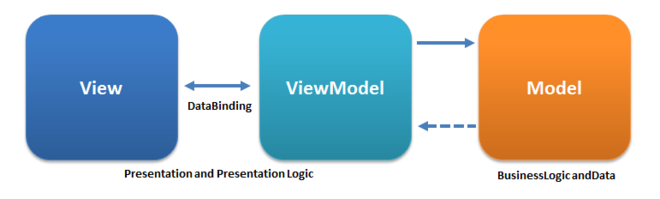
\includegraphics[width=1.0\textwidth]{mvvm}
\centering
\label{fig:reactive-repository}
\caption{MVVM patern architecture }
\end{figure}

\begin{enumerate}
\item Model is the domain object, it represents the actual data 
\item View is the presentation of the data, what the final users see. It allows for interaction to take place, such accepting new input or  modifying already existing data
\item ViewModel is a key piece of the triad on the ground that it introduces Presentation Separation.  Instead of making the model aware of the user’s view of the data, the model simply holds the data, the view just holds the formatted data, and the controller is the one that acts as the liaison between the two. The controller might take input from the view and place it on the model, or it might interact with a service to retrieve the model, then translate properties and place it on the view.
\end{enumerate}

The Data Binding part is where the reactive programming really shines by helping to reduce the event/callback clutter. Also, the ViewModel is outputing an observable so that the user interface can subscribe and automatically updates the changes that occur in the Model.


\begin{figure}[H]
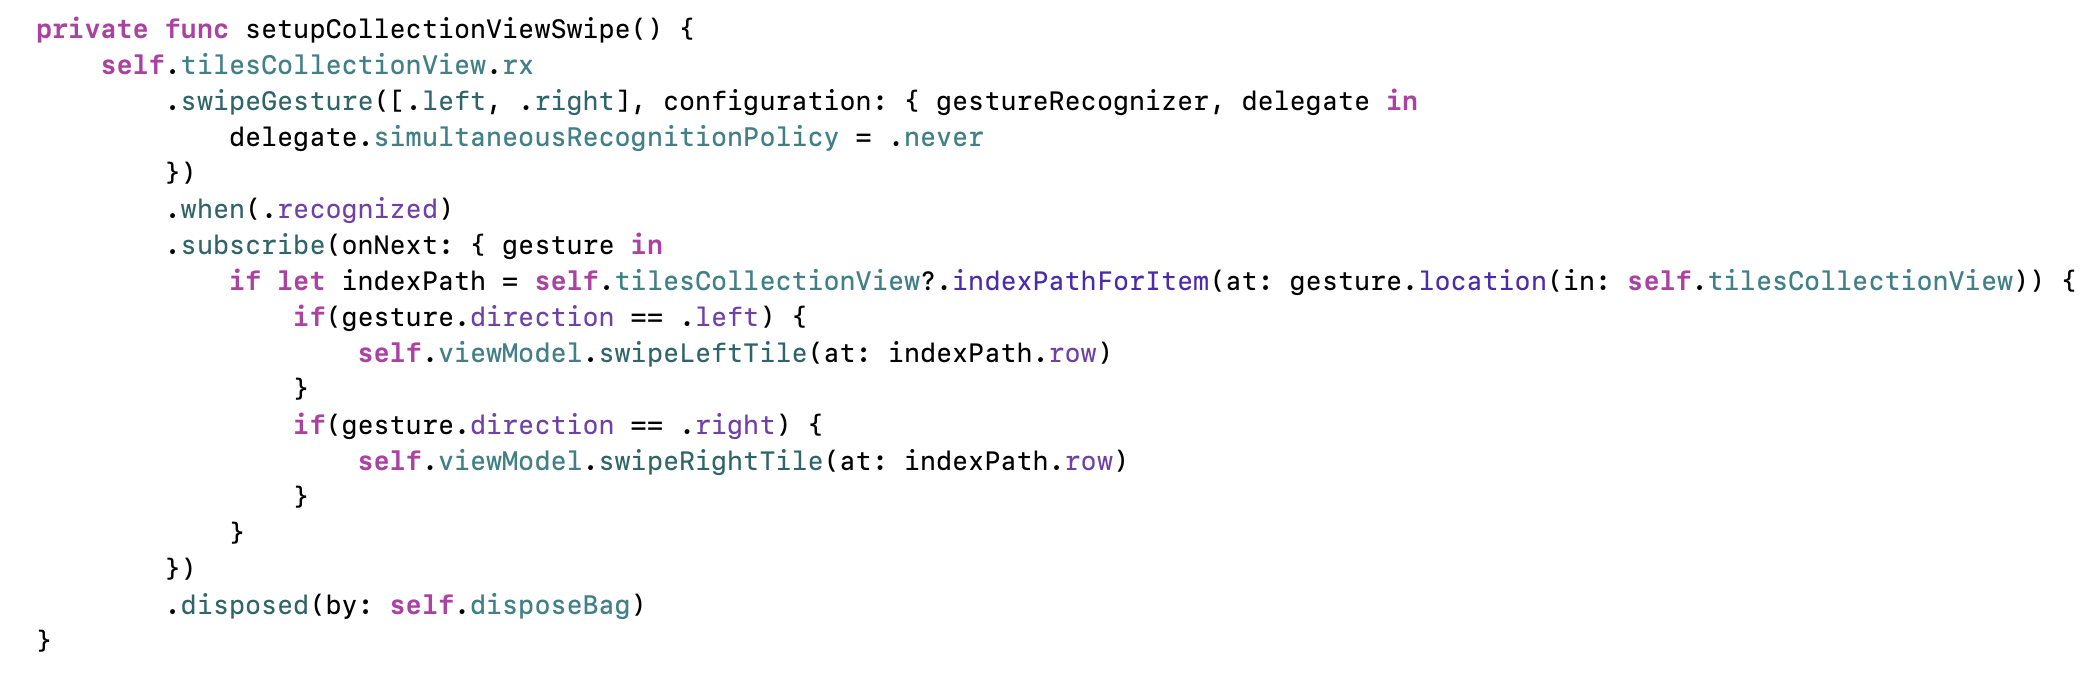
\includegraphics[width=1.0\textwidth]{reactive-ui}
\centering
\label{fig:reactive-repository}
\caption{ Reactive data binding }
\end{figure}

\section{Gamification}
\begin{figure}[H]
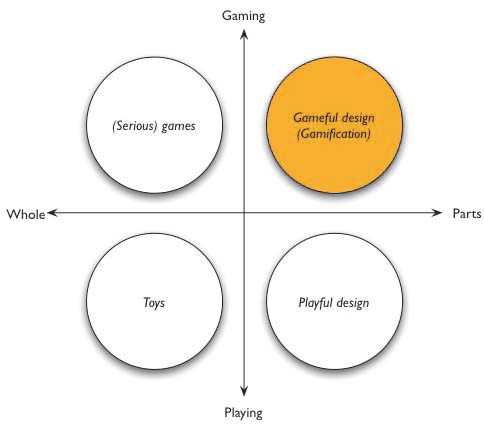
\includegraphics[width=0.65\textwidth]{gamification}
\centering
\label{fig:feature-points}
\caption{ Matrix classifing concepts related to gamification \cite{deterding} }
\end{figure}

As the target public is formed of young kids, packing the application in a form that would appeal to them and that would envelope the learning process into an interactive game represents on of the most important aspects in maximising the impact of such an application. 

At the first look, the aspect of an application is enough to catch the attention of a kid, but especially at these ages, kids have the tendency to be drawn toward new activities rather than sticking to already known ones, but from an educational point of view in order to actually make a difference, the rate of retention is crucial, keeping them focused, motivated and willing to return in the application for the purpose of of completing other levels.


Gamification helps this purpose by offering a collection of techniques:

\begin{enumerate}
\item Games adapt their difficulty to be slightly harder then the player skill
\item The ability to receive items when a certain point has ben reached, in other words this represents a do-reward mechanism
\item Settings a series of goals (through achievements for the case of this application)
\item Integration with real world, augmented reality being a powerful technique
\item The ability to self-express, to either customise certain elements (like the chosen character) or create (through the level builder)
\end{enumerate}
\subsection*{Hero choser}
\begin{figure}[H]
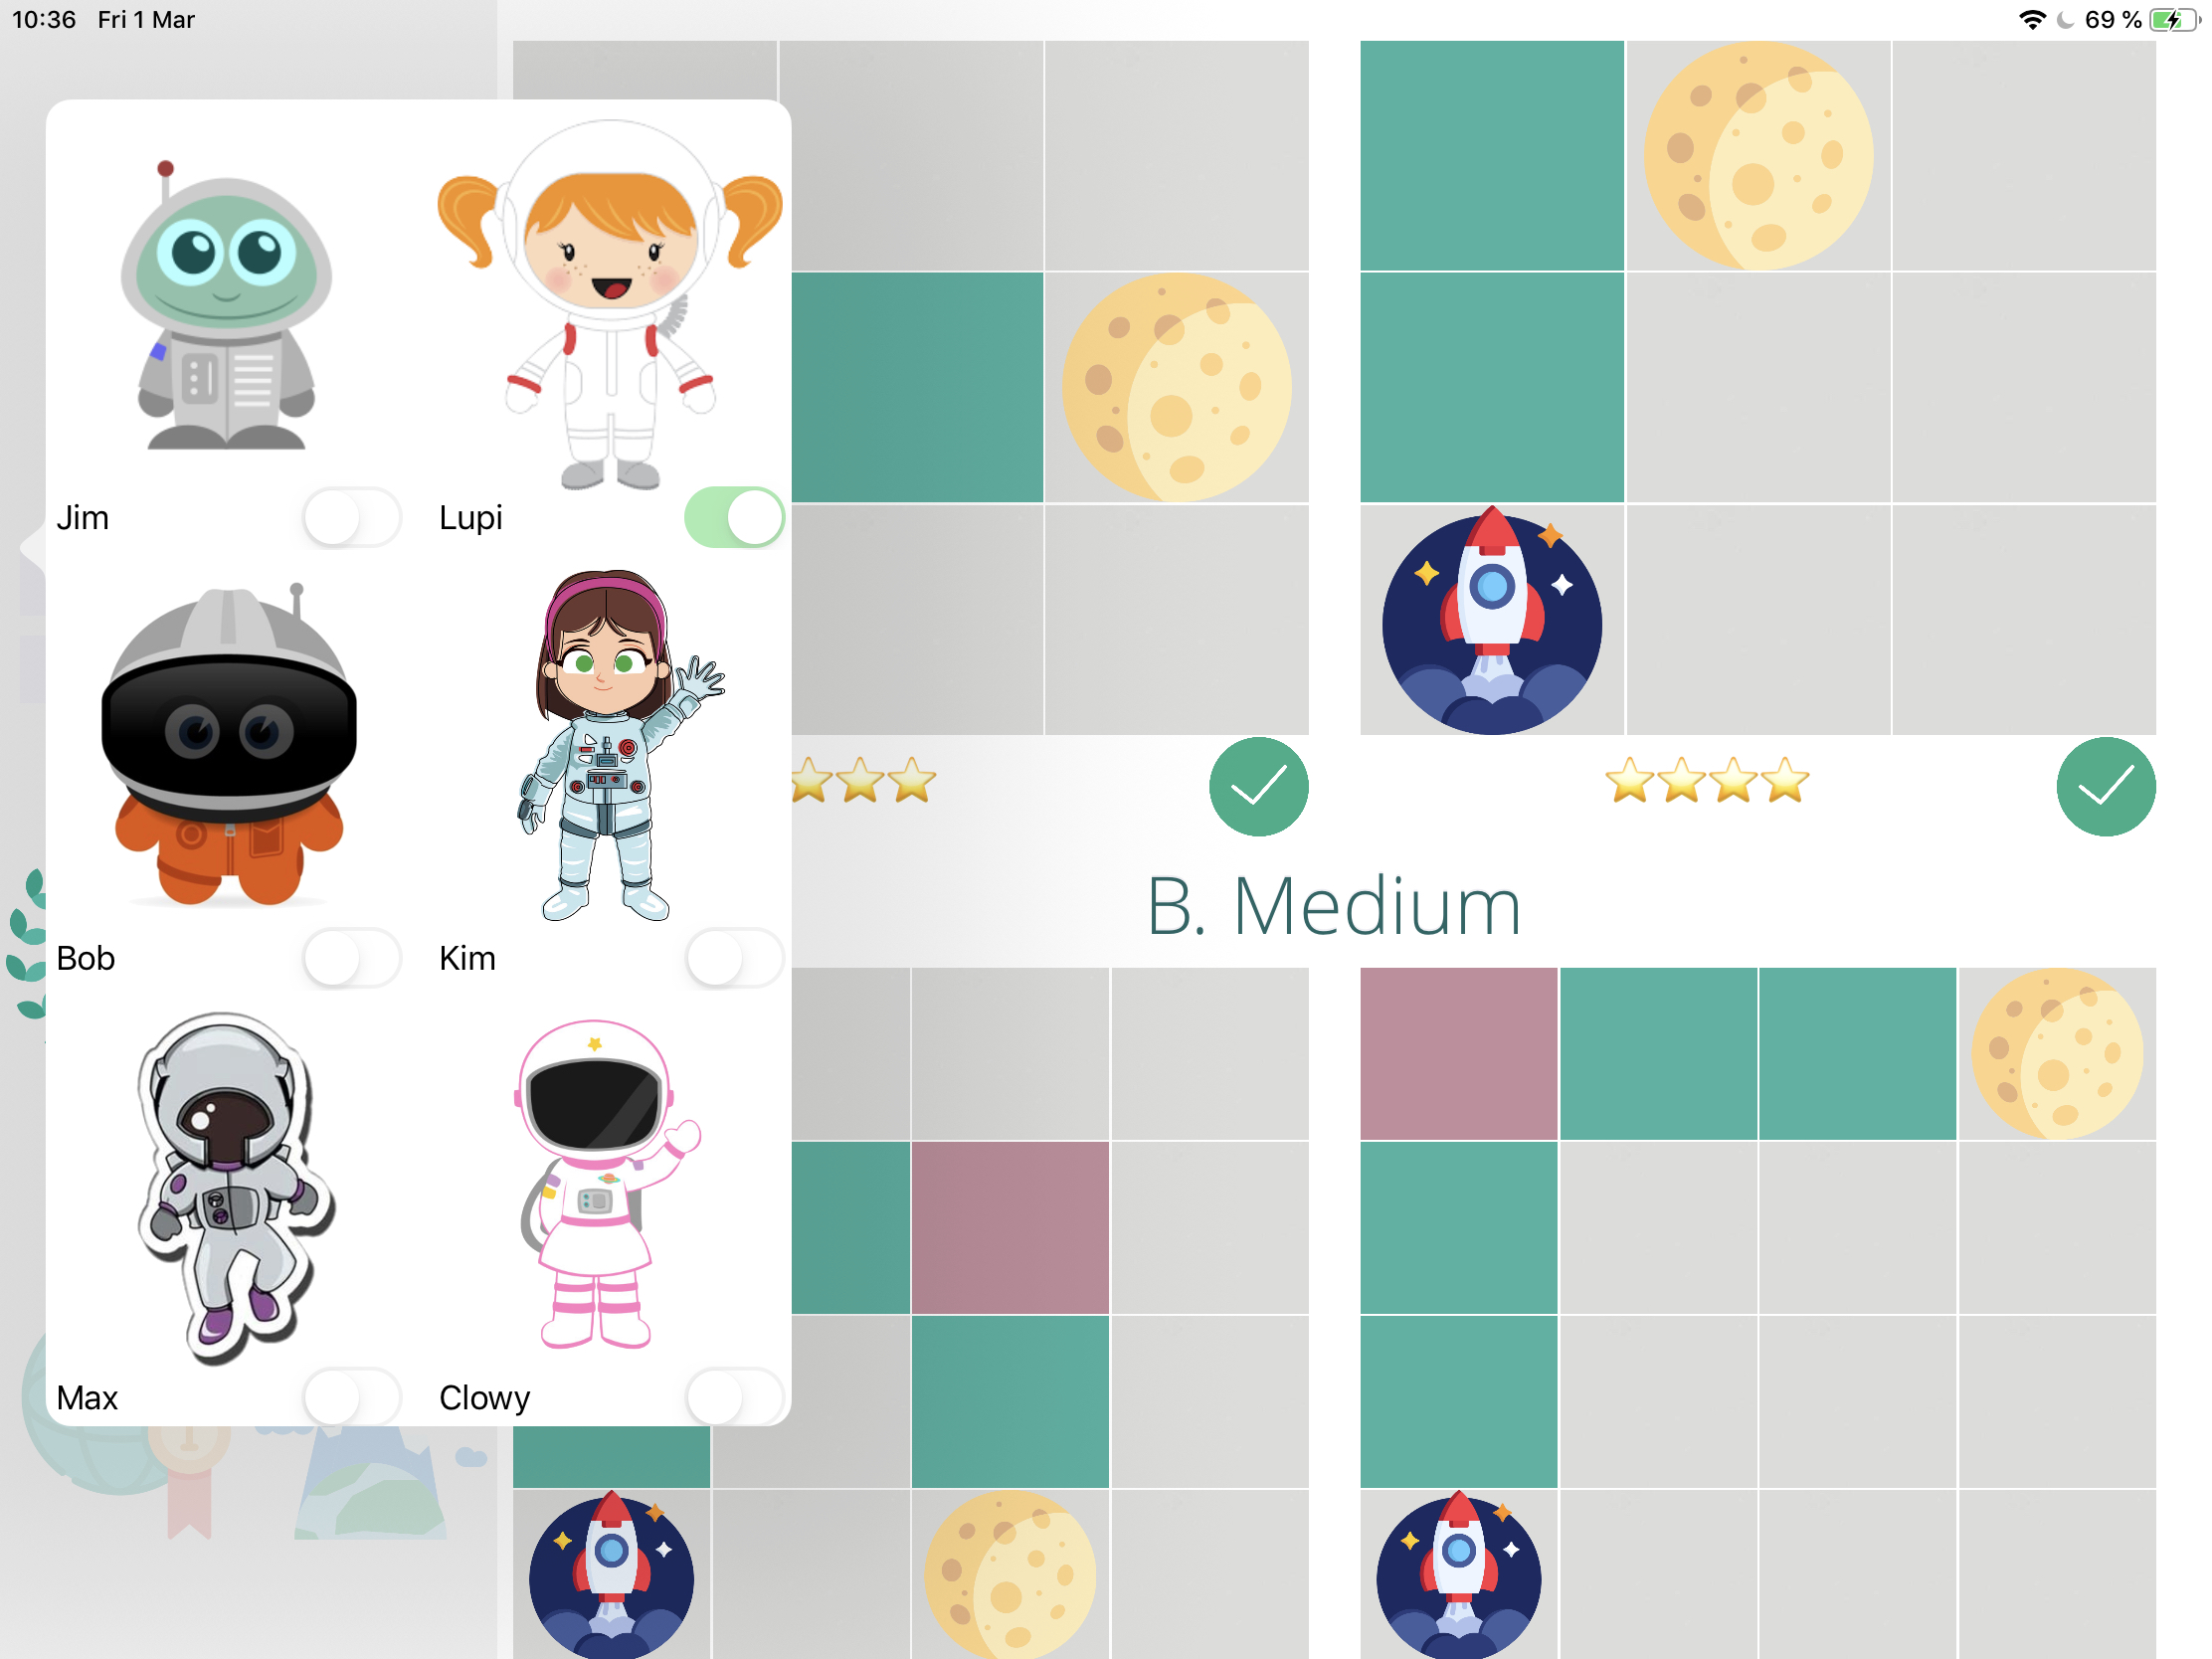
\includegraphics[width=0.89\textwidth]{ArRobotCode1}
\centering
\label{fig:feature-points}
\caption{Interface that enables the process of choosing a hero }
\end{figure}

Unlocking new characters that relates to the personality of the kids is a motivator to continue playing and solving levels so that the risk of abandonment is diminished, and the feeling of accomplishment is stimulated.

Each character has a number of levels that must be successfully completed in order to unlock them.  By default, there are two characters unlocked such that they discover the functionality and realise that more are to be unlocked if they complete enough levels.

The benefits of unraveling a new character are only aesthetic, no actual advantage is being given in the game, but this hasn't proved to negatxively affect the user experience on the grounds of their age.

The aspect of the characters is chosen to reflect the general theme of the game, space exploration, a topic known to attract people of all ages, specially kids.

From a technical point of view the list of characters is shown into a modal window rendering over the Main Activity. Collection View was used as a container rendering two elements per row and in order to allow the selection of different available characters a tap listener is in place for every element showed in the collection view.

\subsection*{Achievements}
 
 \begin{figure}[H]
  \centering
  \begin{subfigure}[b]{0.3\linewidth}
    
\includegraphics[width=\linewidth]{ArRobotCodeAchiv1}
     \caption{For X}
     
  \end{subfigure}
  \begin{subfigure}[b]{0.3\linewidth}
    
\includegraphics[width=\linewidth]{ArRobotCodeAchiv2}
    \caption{For Y}
  \end{subfigure}
  \begin{subfigure}[b]{0.3\linewidth}
    
\includegraphics[width=\linewidth]{ArRobotCodeAchiv3}
    \caption{For Z}
  \end{subfigure}
  \begin{subfigure}[b]{0.3\linewidth}
    
\includegraphics[width=\linewidth]{ArRobotCodeAchiv4}
    \caption{For W}
  \end{subfigure}
  \caption{Achievements}
  \label{fig:coffee3}
\end{figure}

On the ground that the number of completed levels is not the only quantification of the user's progress. Achievements stimulate the usage of certain features of the application in some specific ways that ultimately bring benefsits to the experience of learning.

More specifically, achievements can direct the user to only use certain instructions for some levels (or chapters of levels) so that they are encouraged to find different ways to solve similar problems. Other aspects that can be targeted are the speed of coding, the precision with which they solve challenges (number of tries until their code is correct).

\section{Conclusion}

\chapter{Conclusion}
Final conclusionss!




\begin{thebibliography}{3}
\bibitem{note1}
Saidin, Nor and Abd halim, Noor and Yahaya, Noraffandy. (2015). A Review of Research on Augmented Reality in Education: Advantages and Applications. International Education Studies. 8. 10.5539/ies.v8n13p1. 
\bibitem{note2}
Popelka, Ondřej and Procházka, David and Kolomaznik, Jan and Landa, Jaromir and Koubek, Tomas. (2012). Adaptive Real-Time Object Recognition for Augmented Reality. 
\bibitem{note3}
Silva, Rodrigo and Rodrigues, Paulo and Mazala, Diego and Giraldi, Gilson. (2004).Applying Object Recognition and Tracking to Augmented Reality xfor Information Visualization. 
\bibitem{note4}
Kesim, Mehmet and Ozarslan, Yasin. (2012). Augmented Reality in Education: Current Technologies and the Potential for Education. Procedia - Social and Behavioral Sciences. 47. 297–302. 10.1016/j.sbspro.2012.06.654. 
\bibitem{reactivexDocumentation}
ReactiveX documentation 2019. [Online; accessed 2-May-2019]
\bibitem{deterding}
Deterding, S., Sicart, M., Nacke, L., O'Hara, K., & Dixon, D. (2011b). Gamification. Using Game-Design Elements in Non-Gaming Contexts. In CHI'11 Extended Abstracts on Human Factors in Computing Systems (pp. 2425-2428).
\end{thebibliography}


\end{document}